This chapter begins by determining the sensitivity of the search strategy as a function
of the masses and the lifetimes
of the exotic particles. That discussion is followed by a description
of the reconstruction of long-lived dijet candidates.
The signal and background candidates are examined using simulated samples followed by 
a correlation study between the discrimination criteria.

\section{Signal model sensitivity}
\label{sec:sigsensitivity}

\subsection{\Higgs mass}

The \Higgs mass range sensitivity is mostly affected by the $H_T>300\GeV$ requirement imposed by the trigger. 
In order to minimize the effects of the trigger turn-on curve,
we require $H_T>325\GeV$ in the offline reconstruction.

\begin{figure}[htbp]
\centering
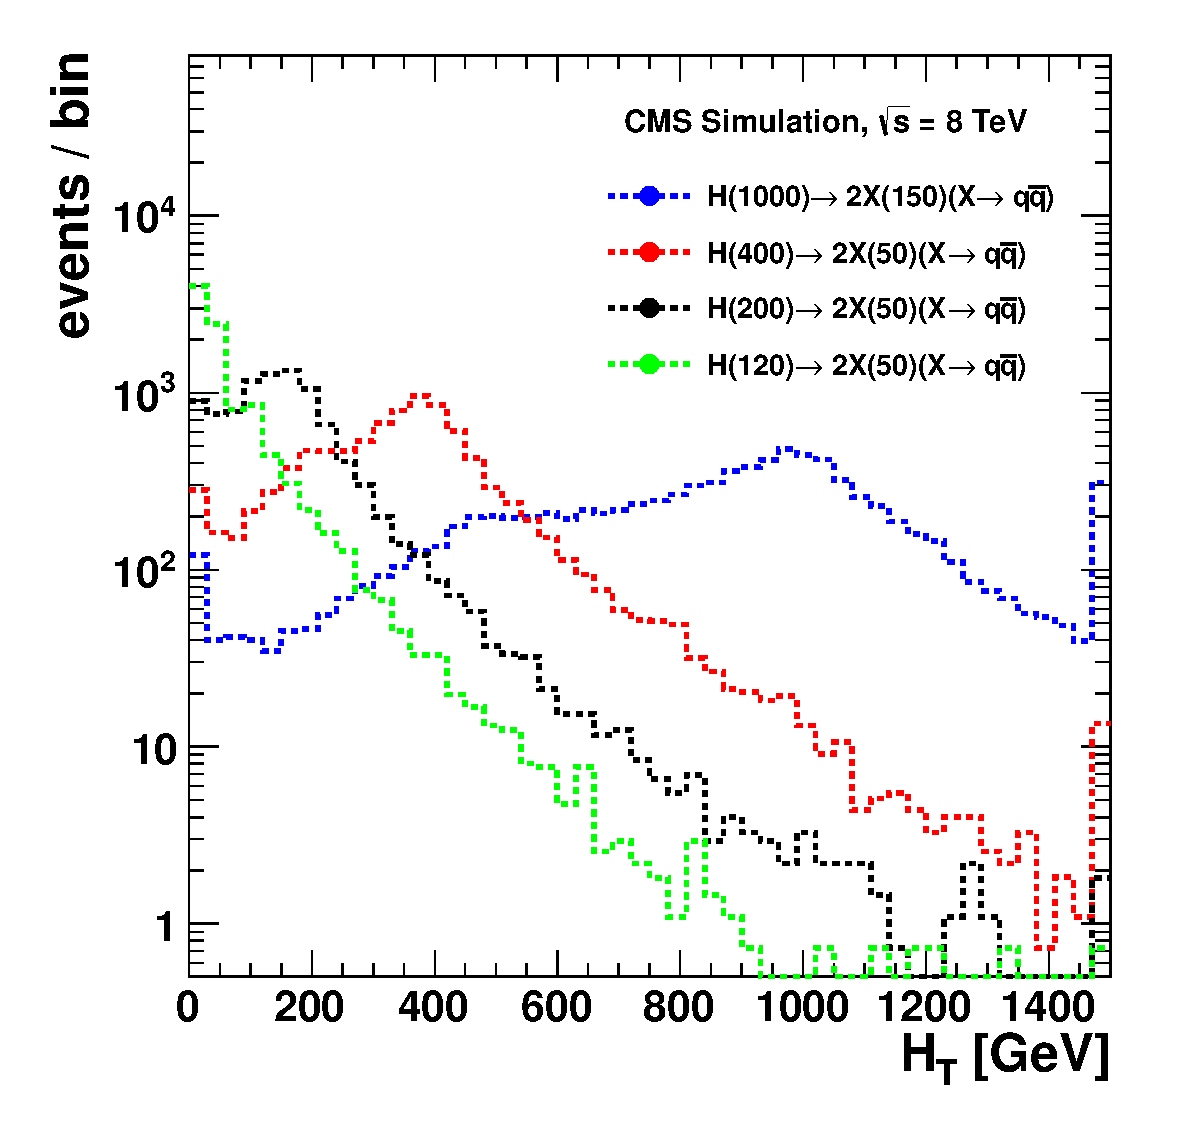
\includegraphics[width=0.49\textwidth]{plots/signal/ht.pdf}
\caption{$H_T$ distributions for the benchmark signal models.\label{fig:sight}}
\end{figure}

Figure \ref{fig:sight} presents the offline reconstructed $H_T$ distributions 
for selected signal models; all available \Higgs 
mass points are shown.
The $H_T>325\GeV$ requirement reduces the sensitivity of the search in the low mass region of the exotic \Higgs,
therefore we analyze further only those signal models where mass of the \Higgs is 200\GeV or higher.

\subsection{\X mass given the \Higgs mass}

In this search we aim to reconstruct displaced dijet candidates originating from a common displaced
vertex using pairs of 
 jets which need to fall 
within the tracker acceptance ($|\eta|<2$).  
 The jets are reconstructed with an anti-k$_T$
algorithm operated with a size parameter $R$ of 0.5 \cite{Cacciari:2008gp} which also determines
the minimal angular distance between the jets reconstructed in the event. 
In order to reconstruct two distinct
jets with this algorithm the opening angle between the two quarks needs to be above 0.5 radians.
Figure \ref{fig:sigdR} presents the opening angle distributions between the two quarks originating
from $\X \to \qq $ decay for signal models with 
$M_{\Higgs}$= 200, 400, 1000\GeV.  

\begin{figure}[htbp]
\centering
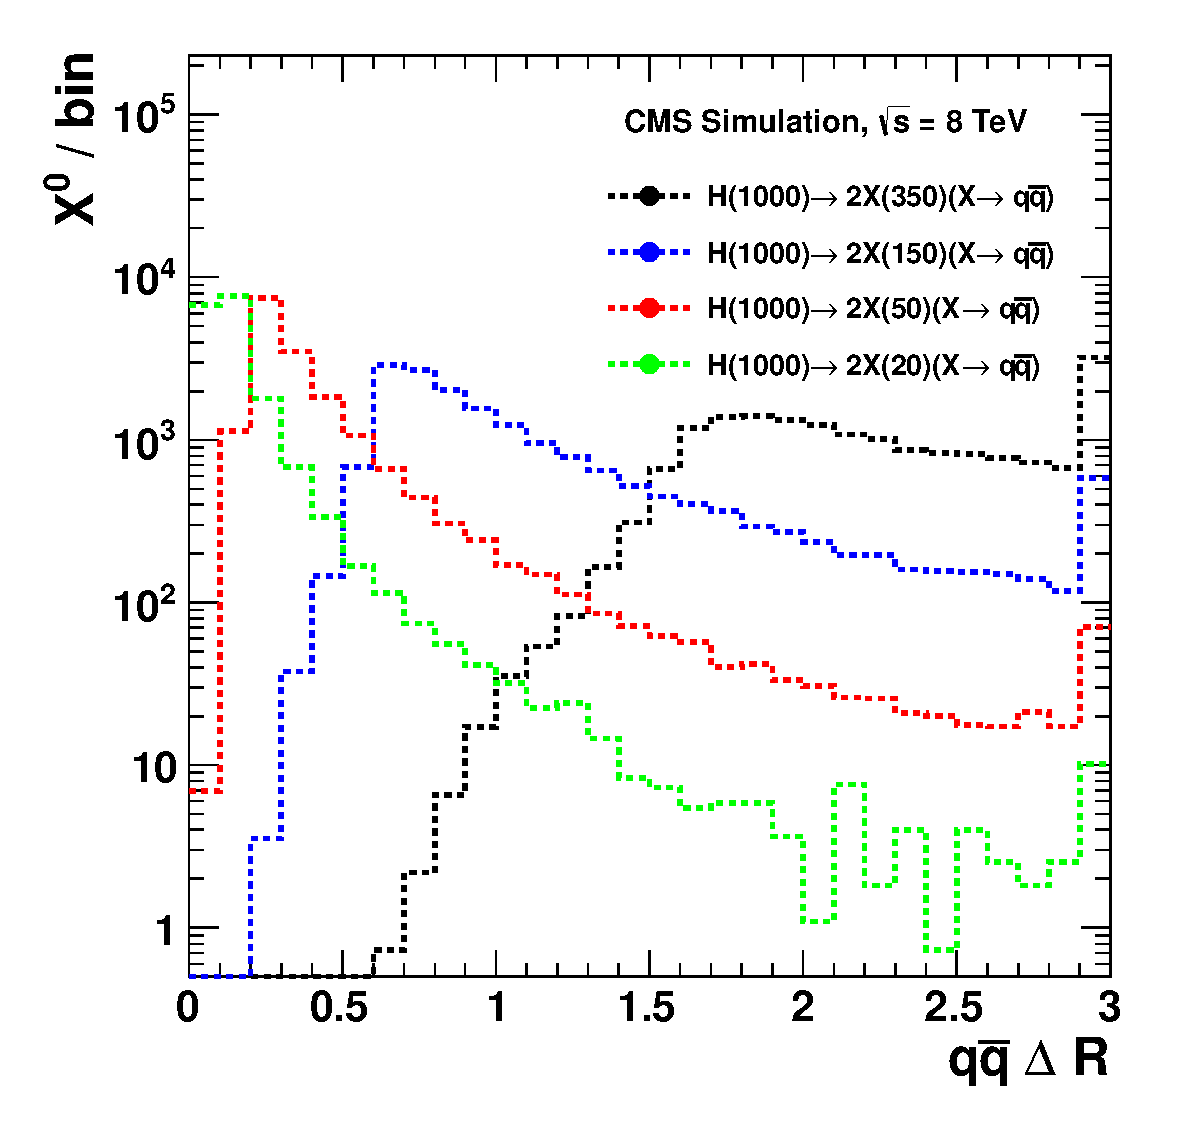
\includegraphics[width=0.49\textwidth]{plots/signal/dRH1000.pdf}
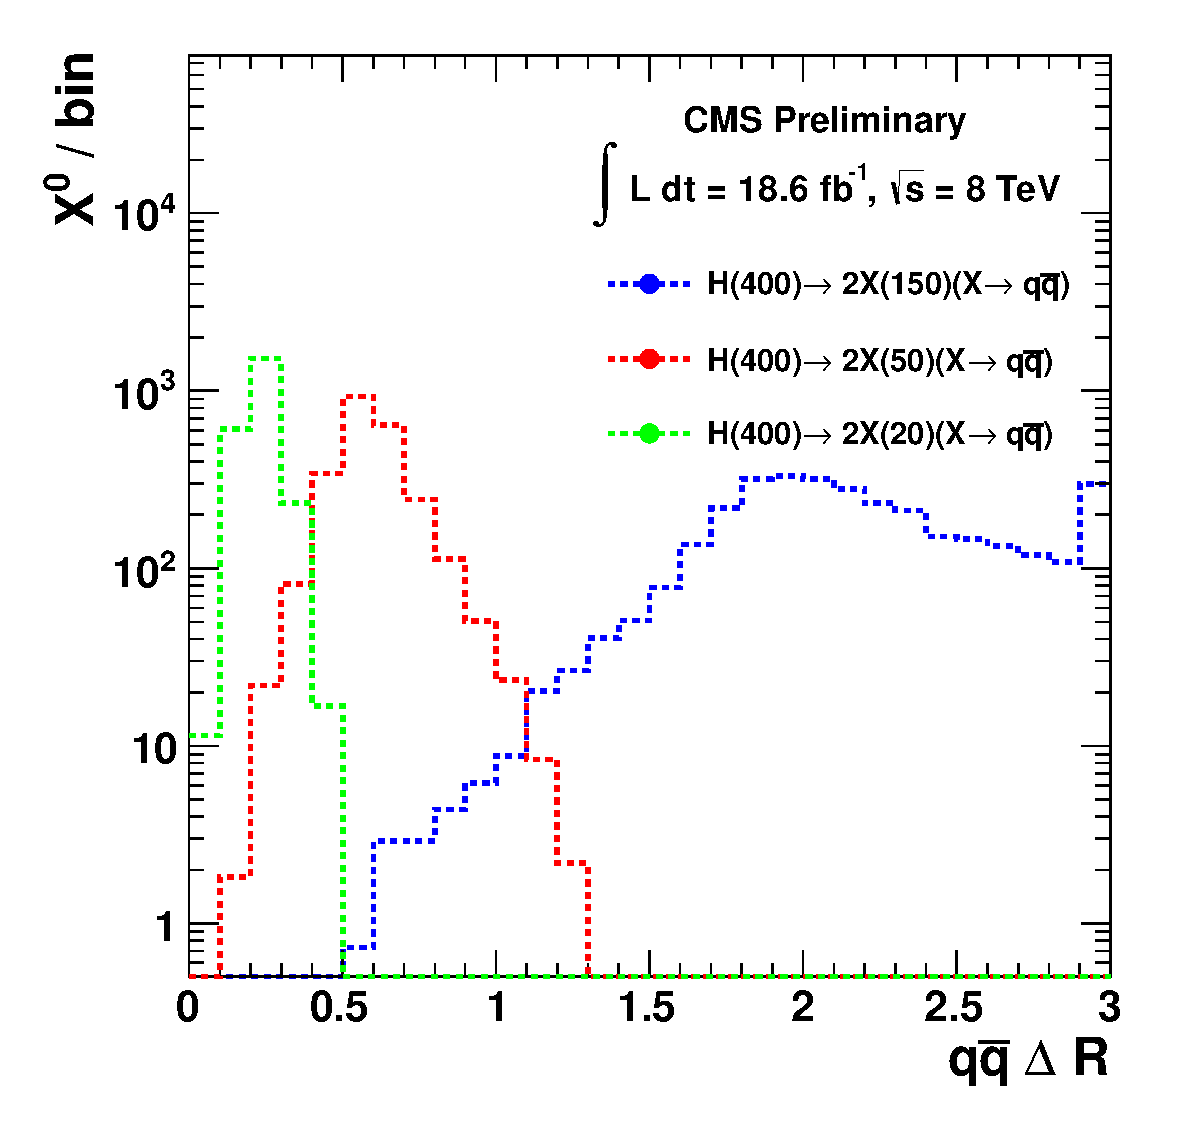
\includegraphics[width=0.49\textwidth]{plots/signal/dRH400.pdf}
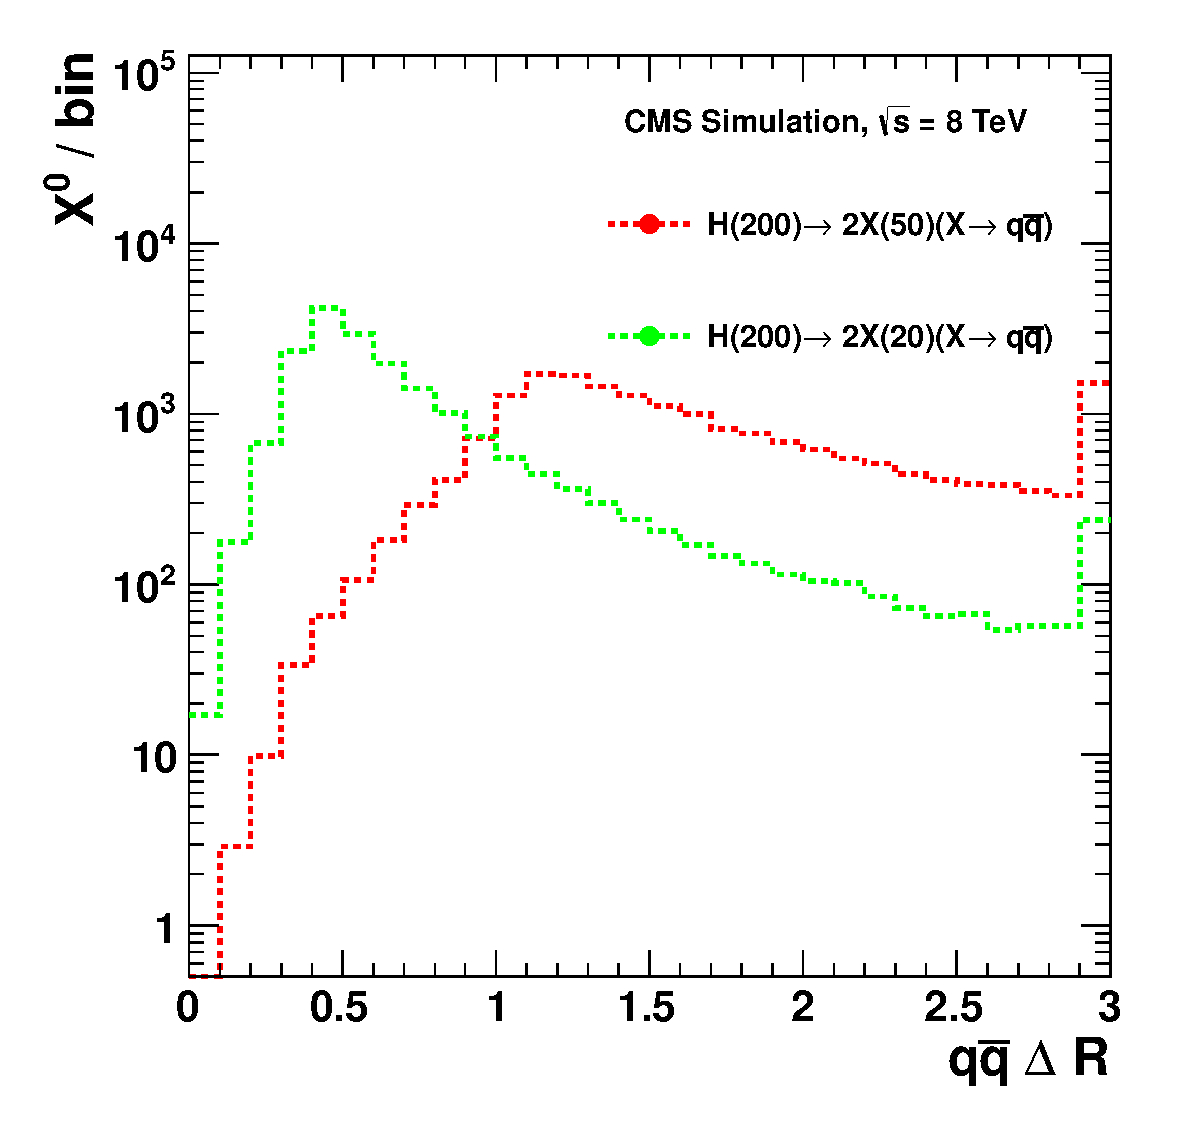
\includegraphics[width=0.49\textwidth]{plots/signal/dRH200.pdf}
\caption{Opening angle distributions of the $\qq$ pair originating from the $\X \to \qq$ decay as a function
of \Higgs and \X particles masses. \label{fig:sigdR}}
\end{figure}

\begin{figure}[htbp]
\centering
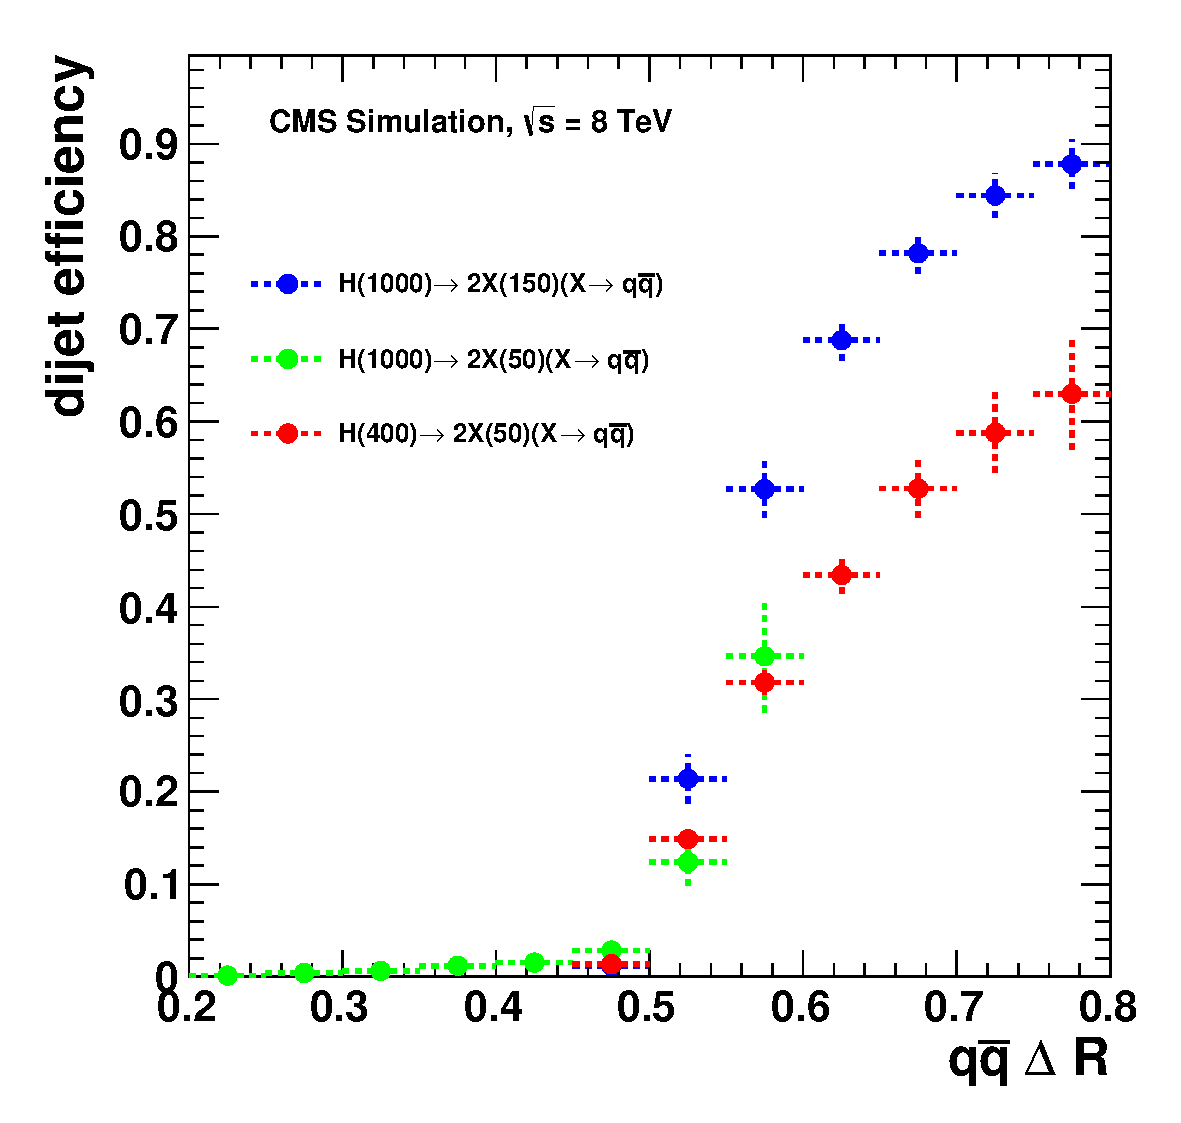
\includegraphics[width=0.49\textwidth]{plots/signal/effDijet.pdf}
\caption{Dijet reconstruction efficiency as a function of the quark-pair opening angle for jets reconstructed with an
anti-k$_T$ algorithm operated with a cone size of 0.5. Both reconstructed jets are required to have a $p_T>60$\GeV
and $|\eta|<2$.  \label{fig:effdR}}
\end{figure}

The efficiency of reconstructing a pair of jets
 corresponding to the $\X \to \qq$ decay using anti-k$_T$ algorithm with the 0.5 radius as a function of the
opening angle of the quark pair is shown in Figure \ref{fig:effdR}. Both jets are required 
to have the $p_T>60$\GeV and $|\eta|<2$, which causes the 
efficiency to be reduced for lower \Higgs  mass models.
 

The dijet analysis is therefore sensitive to long-lived \X particles with masses
such that a significant fraction of the candidates have opening angles above 0.5, namely:
\begin{itemize}
\item $M_{\X}$ between 150-350\GeV for $M_{\Higgs}$=1000\GeV
\item $M_{\X}$ between 50-150\GeV for $M_{\Higgs}$=400\GeV
\item $M_{\X}$=50\GeV for $M_{\Higgs}$=200\GeV
\end{itemize}

%Given the kinematic constraints we define the following acceptance criteria 
%for the \X candidates at the generator level:
%\begin{itemize}
% \item $\qq$ opening angle above 0.5;
% \item $p_T>40\GeV$ and $|\eta|<2.1$ for both quarks from the $\X \to \qq$ decay;
% \item transverse decay length, $L_{xy}<60\cm$ - the CMS tracker allows for track reconstruction originating at
%a transverse displacement up to 60\cm, therefore secondary vertices with higher displacement cannot be reconstructed.
%\end{itemize}

%The definition of acceptance is introduced as a minimal set of requirements for the search.
%If any of the criteria is not met by the long-lived object, the reconstruction will not succeed.

\section{Reconstruction}

In the reconstruction process described below, we identify characteristic variables
of the long-lived dijet candidates that provide
signal-to-background discrimination using simulated MC samples.    
There is no SM process giving rise to displaced dijet pairs. Jets may,
however, may contain displaced (high impact parameter) tracks originating from B meson decays, nuclear
interactions of charged particles with the tracker material, \Kshort and $\Lambda^0$ decays, etc. These tracks, if 
present for two distinct jets,
may then cross at a displaced location and mimic a common dijet vertex. 

We apply a trigger that only requires $H_T>$300\GeV, but does not require
the presence of at least two jets having few low impact parameter tracks. Such a requirement
yields very low
candidate counts for the background MC samples.
All figures in this Section that show signal and background MC distributions 
are scaled to the total available luminosity
of 18.5\fbinv. 
The cross section of the signal process has been set to 10 $\mu$b for visual purposes.   

%%% primary vertrex
The LHC collision events usually contain many primary vertices corresponding to multiple proton-proton collisions occurring 
in the same bunch crossing.
Among the set of primary vertices, we select the one whose tracks have the highest squared transverse momentum sum.
 The primary vertex position is
then used as a reference point for computing decay lengths and impact parameters. The impact of a wrong
primary vertex assignment on the background yield and the signal reconstruction efficiency is discussed
in Section \ref{subsec:pv}. 


We search for dijet candidates by selecting every pair of jets, where both jets are required
to have $p_T>$ 60\GeV and $|\eta|<$ 2. 
The signal dijet candidates are limited
to those where both reconstructed jets are matched within a cone of 0.5 to generator level quarks originating
 from the \X boson decay. Applying this requirement does not change the signal reconstruction efficiency
once the full selection is applied. 

 
Additionally, tracks reconstructed with 
the CMS iterative tracking
algorithm \cite{Giordano:2012hr} as described in Section \ref{subsec:trackreco},
 are associated within 0.5 cone to both jets. The track momentum vector used for 
the association is evaluated at the point of closest approach to the beam line. Only tracks
with $p_T>$ 1\GeV are considered. Tracks with lower transverse momenta
do not reach the calorimeter system due their strong deflection in the CMS magnetic field. Among the tracks we select a set of {\bf displaced tracks} defined as those with
a transverse impact parameter with respect to the primary vertex greater than 500\micron, which is large enough
to exclude most of the B hadron decay products. 
The individual impact parameters are signed with the sign of the scalar product between
 the dijet momentum and the impact parameter vectors in the transverse plane.
For each jet we also repeat the calculation of variables used in the displaced jet trigger
 using offline reconstruction, namely:

\begin{itemize}
\item the number of prompt tracks - for tracks with impact parameter in 3 dimensions smaller than 300\micron, 
Figure \ref{fig:discprompt}; 
\item the jet energy fraction carried by prompt tracks - for tracks with transverse impact parameter smaller 
than 500\micron, Figure \ref{fig:discprompt}.

\end{itemize} 

\begin{figure}
\centering
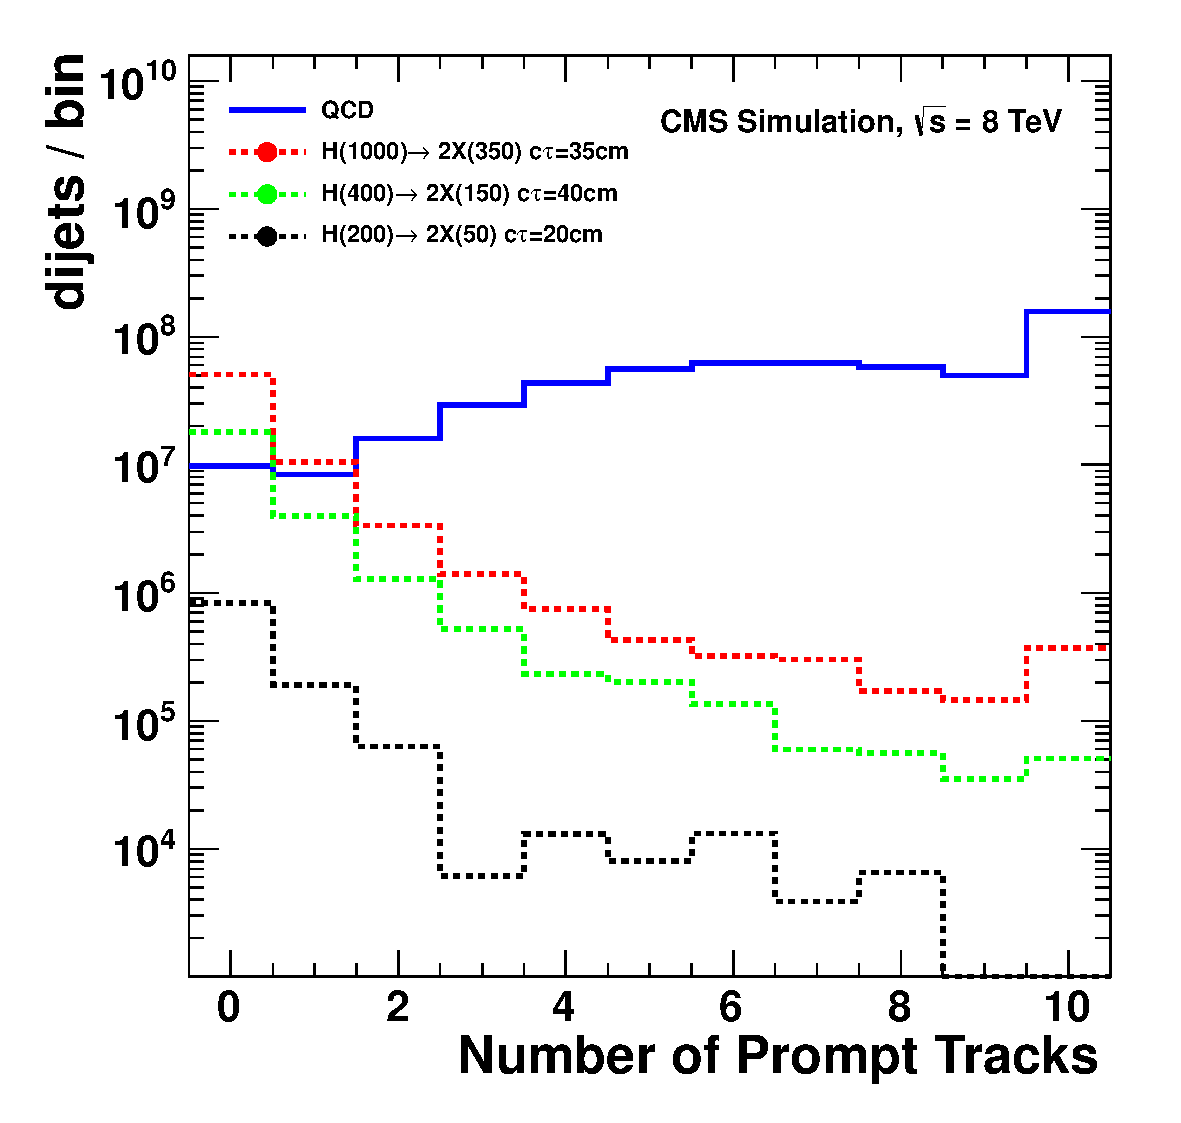
\includegraphics[width=0.49\textwidth]{plots/discrimination/disc_NPromptTracks.pdf}
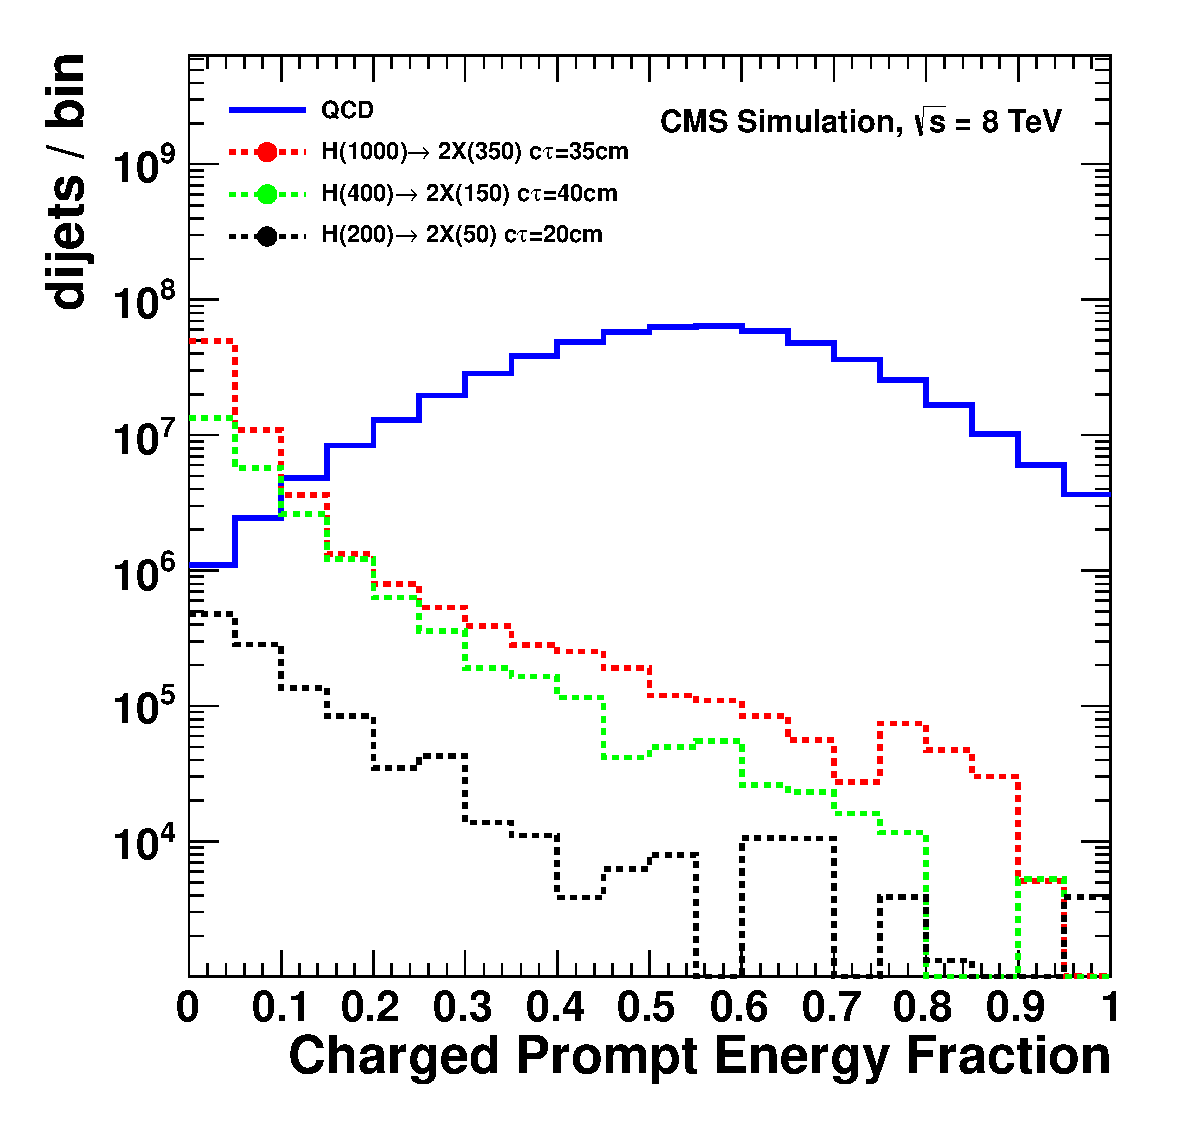
\includegraphics[width=0.49\textwidth]{plots/discrimination/disc_PromptEnergyFrac.pdf}
\caption{Number of prompt tracks associated to the jet and charged prompt jet energy fraction for signal and
background MC samples. There are two jets in a dijet pair, however the distributions for both jets are identical.
We present the distributions for the lower $p_T$ jet in the dijet pair.
\label{fig:discprompt}}

\end{figure}

Secondary vertices are searched among the tracks associated to each dijet pair 
using two different algorithms: 

\begin{enumerate}

\item{\bf Vertex Fitter}
\label{subsec:AVF}
\cite{Waltenberger:1166320}. The fitter performs an iterative least-squares estimation of the
 secondary vertex position. The consecutive iterations down-weight tracks that seem inconsistent
with the fitted vertex position until an optimum is found.
 The secondary dijet vertex is required to have a chisquared per degree of freedom 
$\chi^2/\text{dof} < 5$. Additionally, for compatibility with the displaced dijet hypothesis we require that at least 
one track from each jet be included in the secondary vertex. 
This requirement greatly reduces the background contribution
from nuclear interaction vertices. The nuclear interaction vertices are characterized by low invariant mass
of the outgoing tracks, making it unlikely that the outgoing tracks are associated with
two distinct jets. 
The following quantities obtained from the vertex fit, with plots presented in Figure
\ref{fig:discvtx}, provide discrimination between signal and background:
\begin{itemize}
 \item vertex track multiplicity;
 \item fraction of tracks assigned to the vertex with a positive value of signed impact parameter;
 \item number of missing tracker hits behind the vertex position per track - each track in CMS is reconstructed 
from hits in the silicon tracker using a Kalman Filter algorithm \cite{Giordano:2012hr}. The algorithm propagates
 track seeds through the CMS tracker in the direction from the beam line towards the calorimeters. Whenever a hit 
is found along the trajectory the track parameters are updated, while occasional missing measurements 
are allowed. 
This variable represents an average count of missing tracker measurements 
starting from the fitted vertex position until the innermost hit of the vertex tracks. The fitted vertex position
may be significantly closer to the beam line than the track production point, if the track comes from a nuclear
 interaction or a $V^0$ decay;
 \item invariant mass of the vertex tracks (vertex mass);
 \item $p_T$ of the vertex tracks (vertex $p_T$);
 \item $L_{xy}$ significance - where $L_{xy}$ is the distance between secondary and primary vertices
in the transverse plane.
\end{itemize}


\begin{figure}
\centering
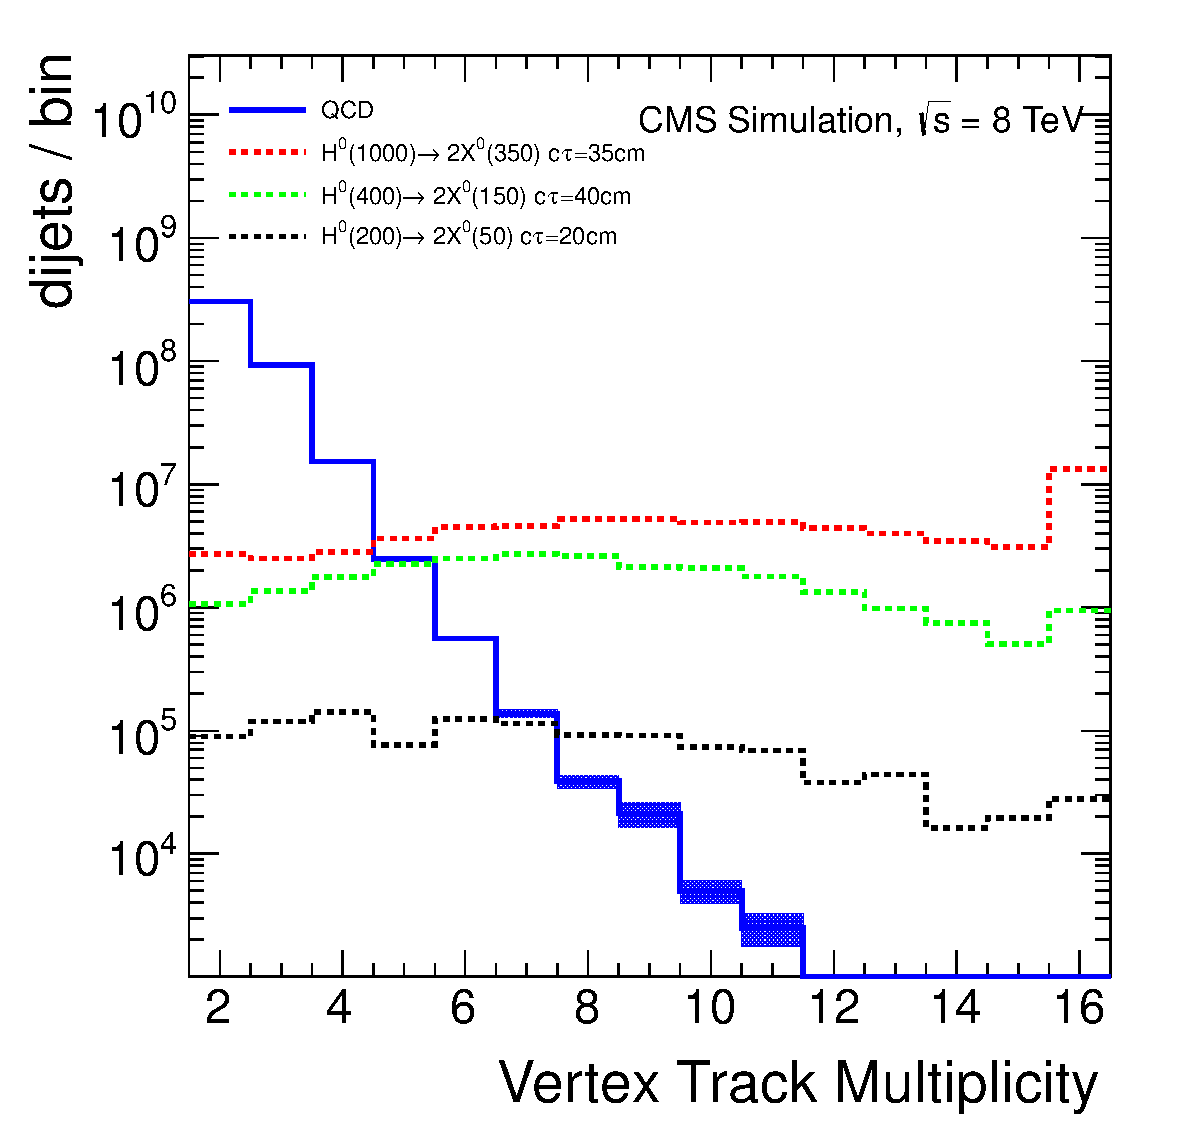
\includegraphics[width=0.49\textwidth]{plots/discrimination/disc_vtxN.pdf}
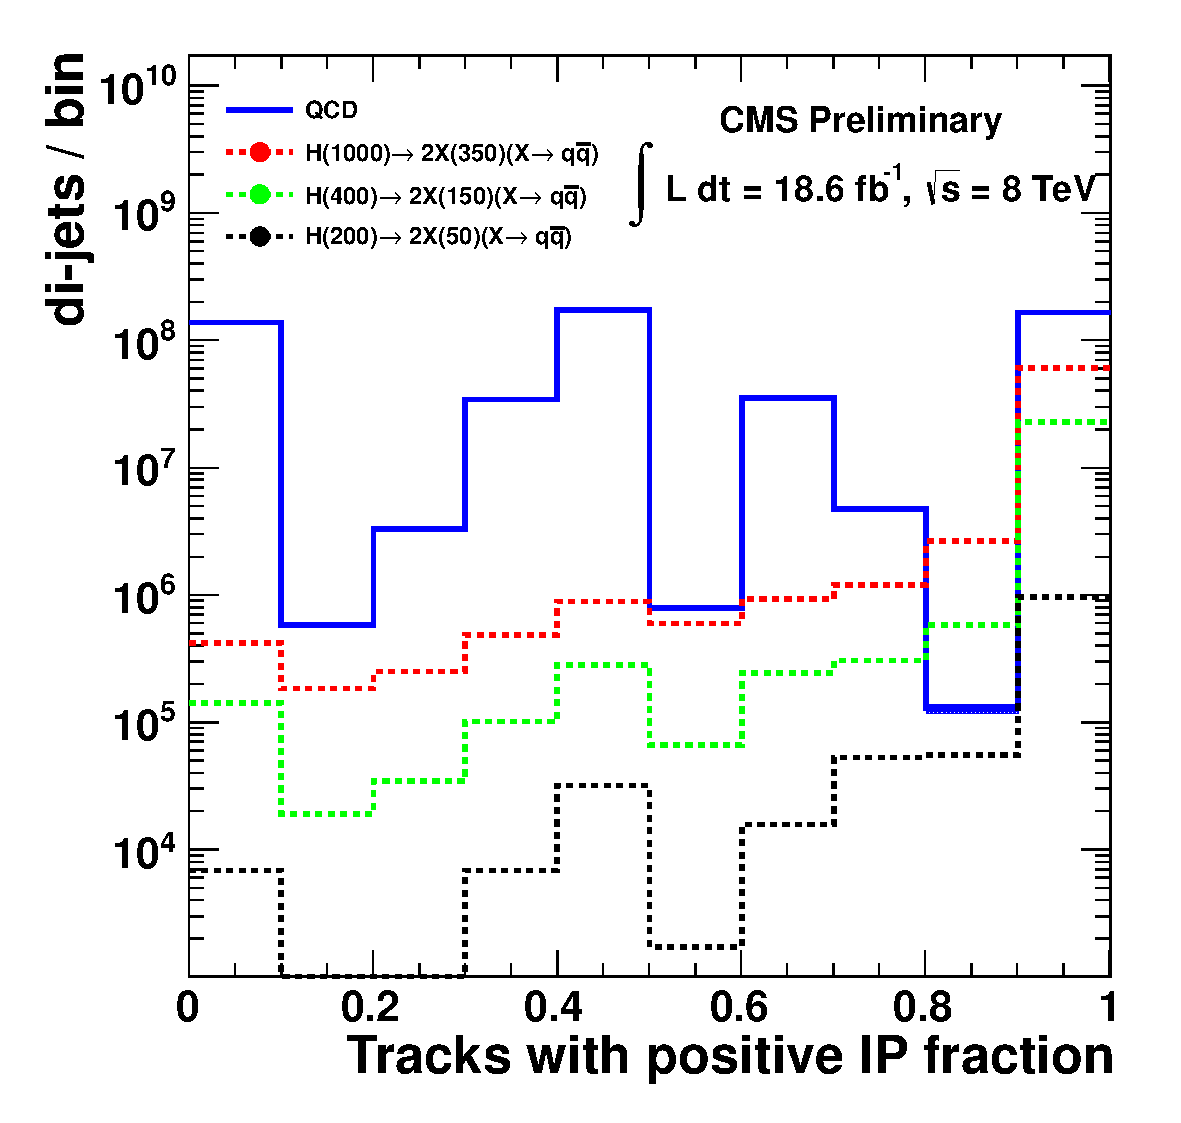
\includegraphics[width=0.49\textwidth]{plots/discrimination/disc_Posip2dFrac.pdf}
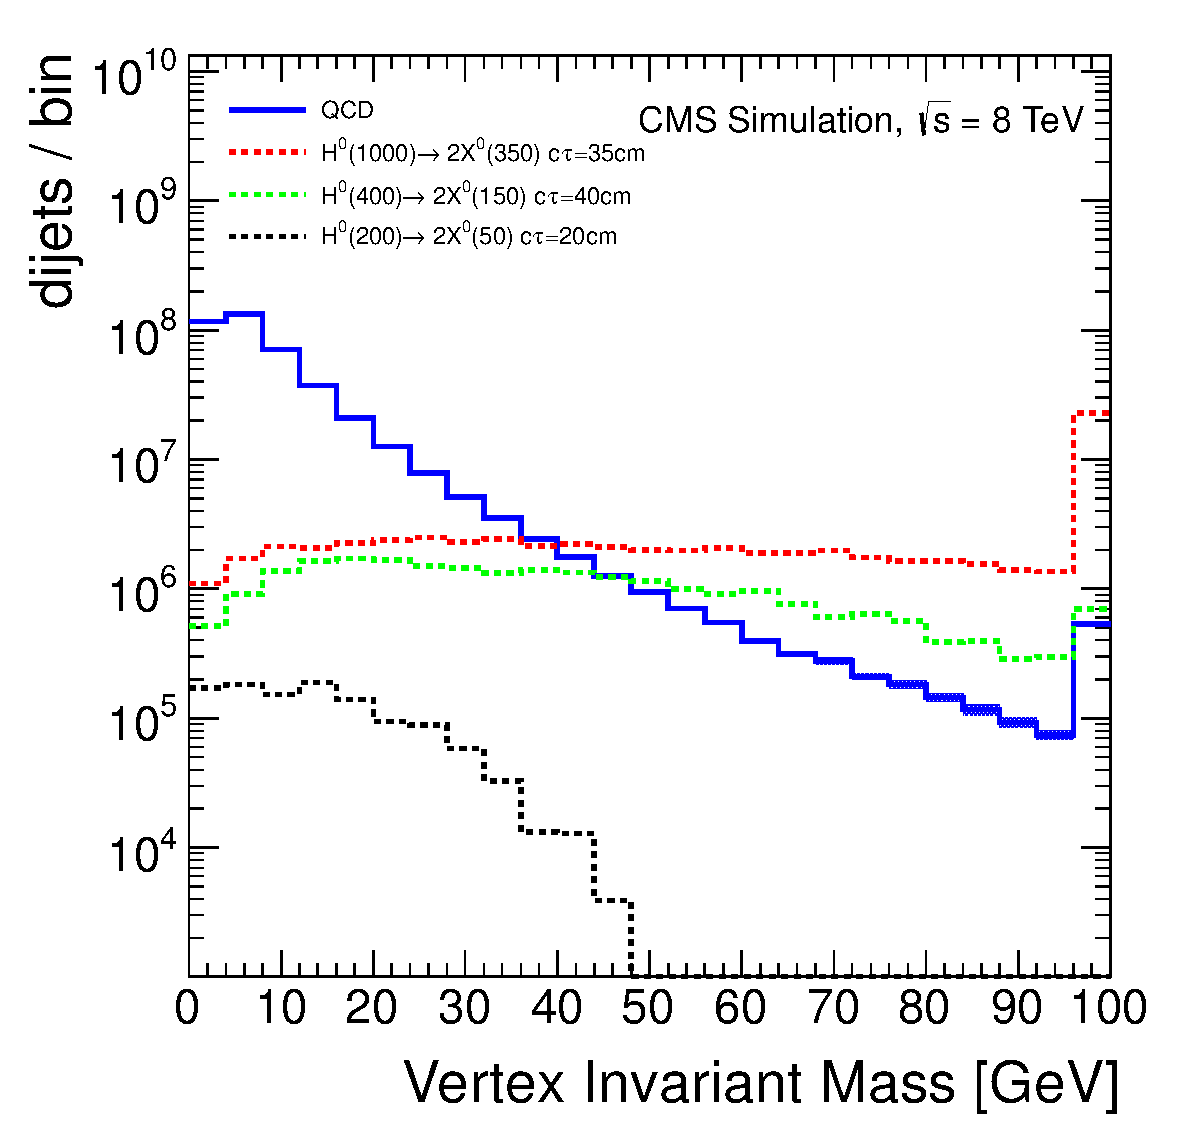
\includegraphics[width=0.49\textwidth]{plots/discrimination/disc_vtxmass.pdf}
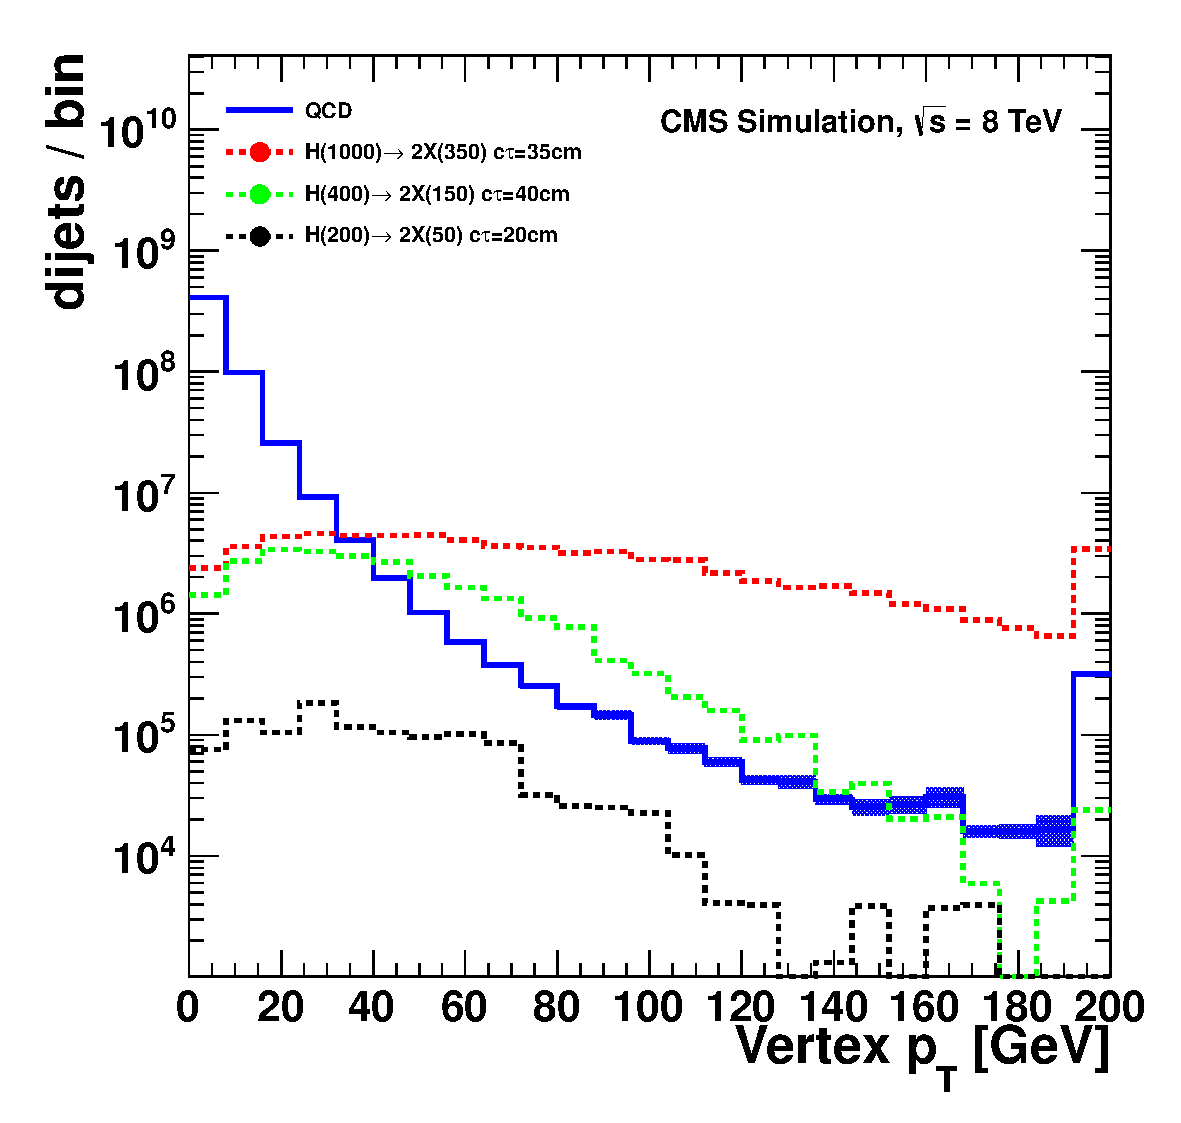
\includegraphics[width=0.49\textwidth]{plots/discrimination/disc_vtxpt.pdf}
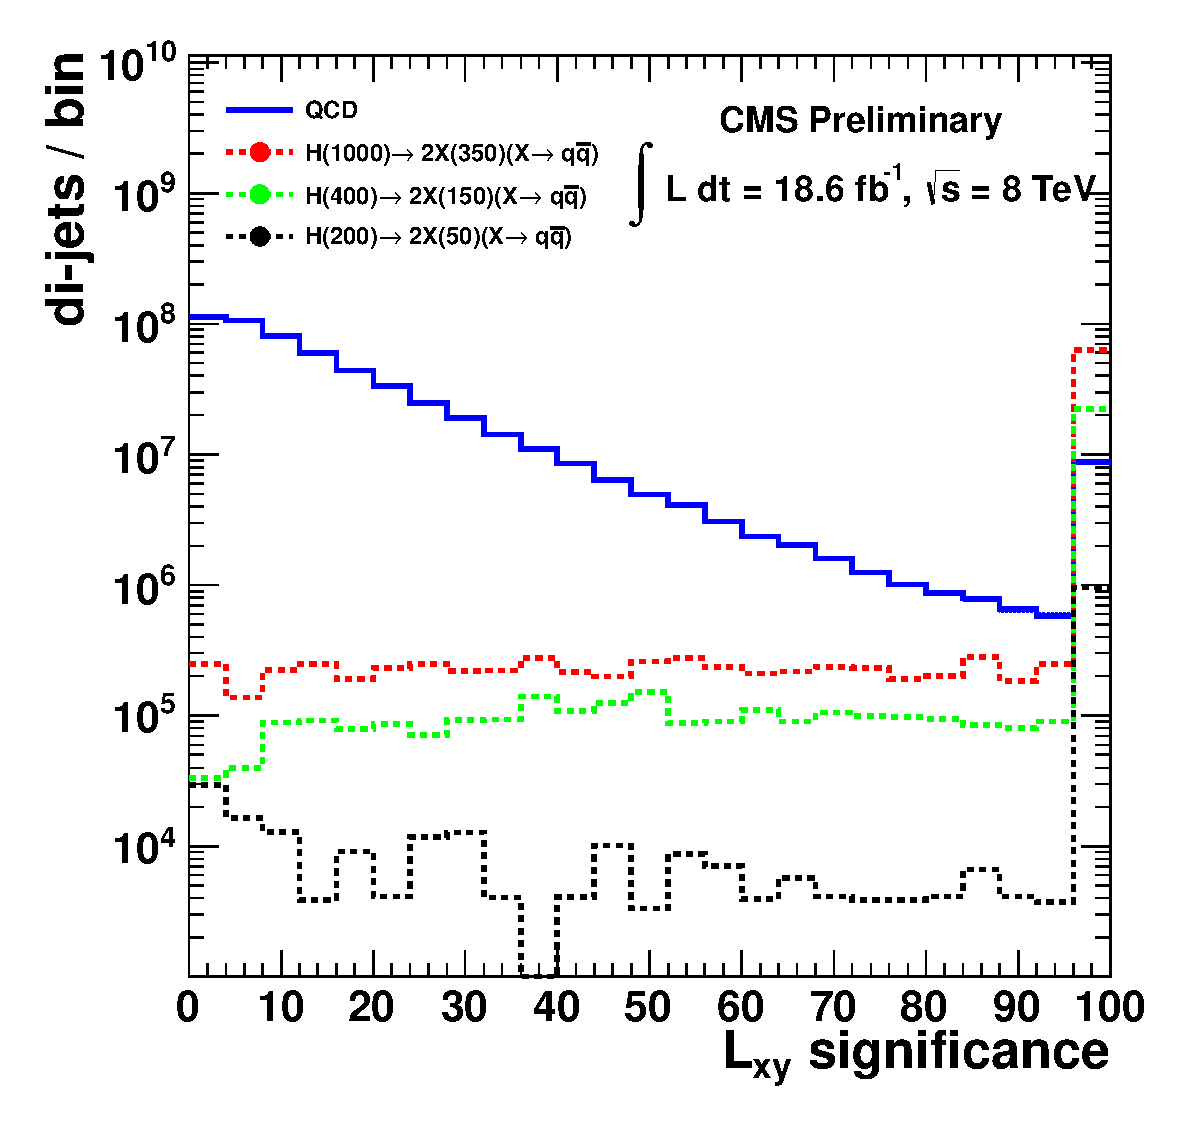
\includegraphics[width=0.49\textwidth]{plots/discrimination/disc_lxysig.pdf}
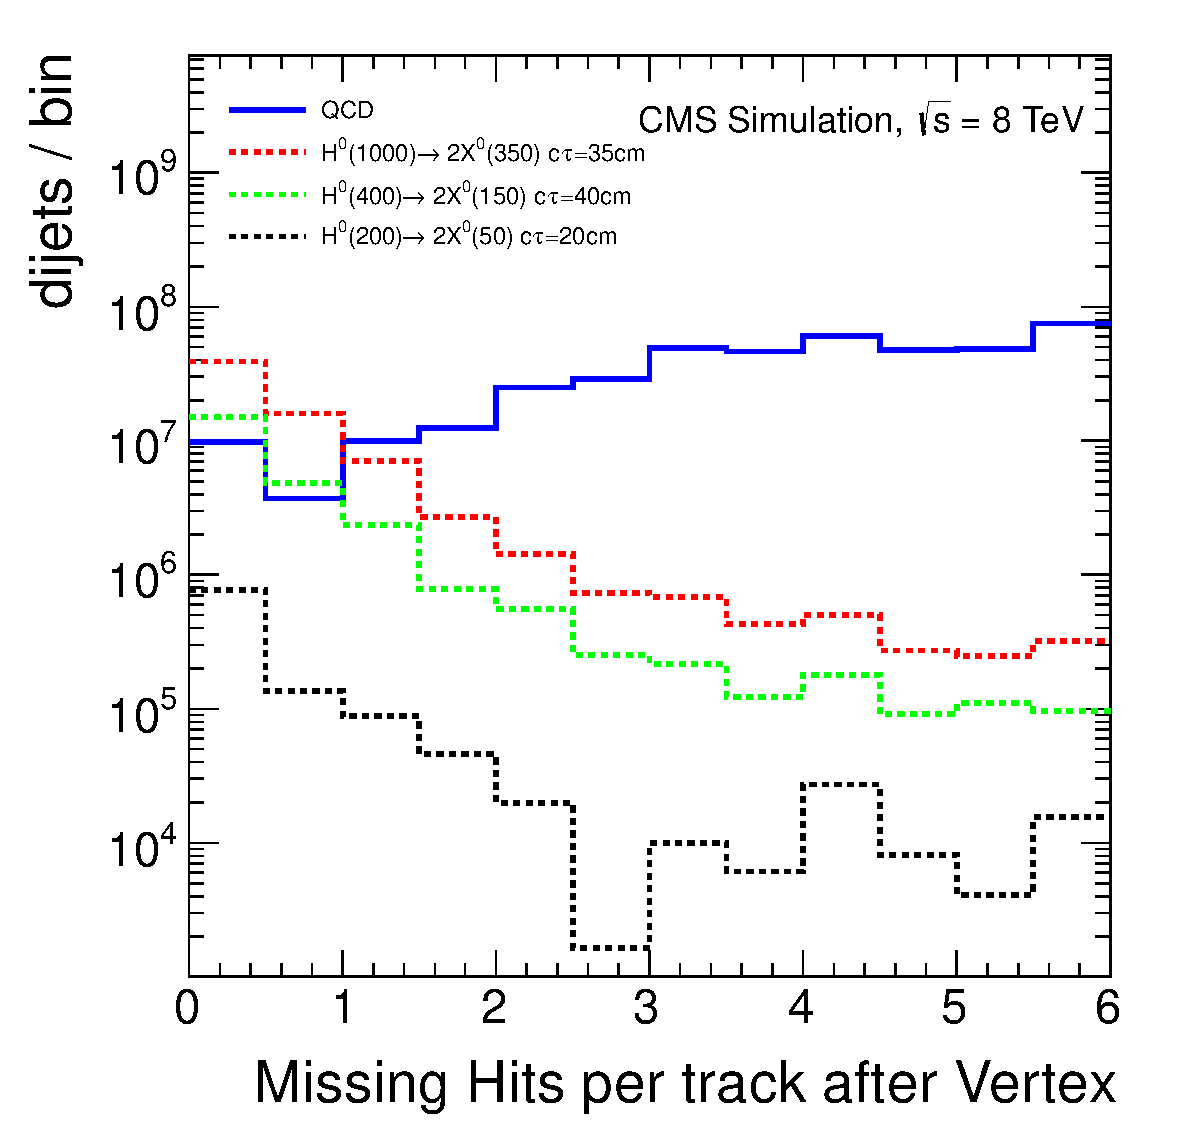
\includegraphics[width=0.49\textwidth]{plots/discrimination/disc_NAvgMissHitsAfterVert.pdf}
\caption{Secondary vertex discrimination variables for signal and background MC samples.\label{fig:discvtx}}

\end{figure}

\item{\bf Clusters of the expected path length}  
\label{subsec:Clusters}
- in this algorithm, for each of the displaced tracks associated with either jet, a decay point consistent 
with the displaced dijet hypothesis 
is determined. As schematically presented in Figure 
\ref{fig:guesslxydiagram} such a point 
 can be obtained as the crossing point of   
the particle trajectory and a straight line drawn from the primary vertex in the direction of the dijet momentum.  
Information about the production point for each track is then used to compute an expected path length in the
transverse plane, $L_{xy}^\text{exp}$.  
For high momentum tracks the trajectory in the transverse plane is a straight line,
 therefore the decay point can be determined from the crossing point between two lines
 and the expected path length is simply:
\begin{equation}
 L_{xy}^\text{exp}=\frac{d_{xy}}{\sin(\phi_\text{track} - \phi_\text{dijet})}
\label{eqn:lxystraight}
\end{equation}
where $d_{xy}$ is the transverse impact parameter and $\phi$ is the polar angle. However, 
in the presence of an axial magnetic field, the formula above is not valid as a result of
curvature. In order to find the expected path length in such cases,
 we find a corresponding crossing point for the track helix with a radius $R$. Since we consider only
tracks with $p_T>$1\GeV, which translates to the helix radius $R$ above 80\cm, 
the calculation is limited to first order in 
$d_{xy}/R$. 
 A line drawn from the primary vertex along the dijet momentum crosses the helix twice, yielding
 two solutions, although only one of them behaves properly when $R \to \infty$ 
and reduces to Eq. \ref{eqn:lxystraight}. Nevertheless, we consider two  
separate cases:
\begin{itemize}
 \item primary vertex lies inside the track helix:
\begin{equation}
 L_{xy}^\text{exp} = \frac{d_{xy}}{\sin\left(\phi_\text{track} - \phi_\text{dijet}\right)} \left(1 - \frac{d_{xy}}{R}\right) + o\left(\left(\frac{d_{xy}}{R}\right)^2\right)
\end{equation} 
 \item primary vertex lies outside of the track helix:
\begin{equation}
 L_{xy}^\text{exp} = \frac{d_{xy}}{\sin\left(\phi_\text{track} - \phi_\text{dijet}\right)} \left(1 + \frac{d_{xy}}{R}\right) + o\left(\left(\frac{d_{xy}}{R}\right)^2\right)
\end{equation} 
\end{itemize}
The difference between the two cases above lies only in the sign of the track curvature correction. This sign,
however,  can be
determined from the track charge and the vector product between the track transverse momentum vector and transverse
impact parameter vector:
\begin{equation}
q\cdot sgn\left(\left(\vec{d_{xy}}\times\vec{p_T}\right) \cdot \vec{z}\right)
\end{equation}   
where $\vec{z}$ is a unit longitudinal vector. The final formula applied to each track is thus:
\begin{equation}
 L_{xy}^\text{exp} = \frac{d_{xy}}{\sin\left(\phi_\text{track} - \phi_\text{dijet}\right)} \left(1 + q\cdot sgn\left(\left(\vec{d_{xy}}\times\vec{p_T}\right) \cdot \vec{z}\right) \cdot \frac{d_{xy}}{R}\right)
\label{eqn:lxy}
\end{equation}


\begin{figure}
\centering
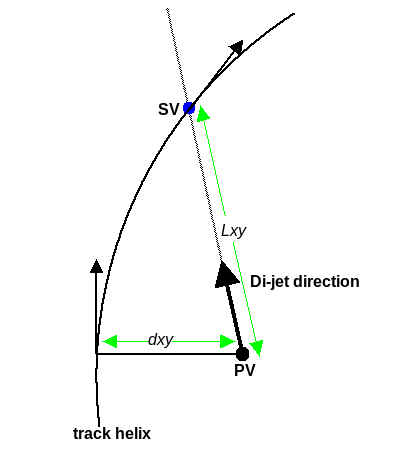
\includegraphics[width=0.3\textwidth]{plots/guessLxy.png}
\caption{Graphical representation of the crossing point (SV) between track helix and a straight line originating from the primary vertex (PV) in the direction of the dijet momentum. \label{fig:guesslxydiagram}}
\end{figure} 

For a genuine secondary vertex associated with a dijet pair the $L_{xy}^\text{exp}$ values obtained with Eq.
\ref{eqn:lxy} for each track should be close
 together, therefore we perform a one-dimensional hierarchical clustering algorithm (Appendix 
\ref{app:clusters})
in order to select tracks belonging to the cluster. 
Clustering is performed with a size parameter equal to 15\% of 
the vertex $L_{xy}$ reconstructed with the vertex fitter. 
The tracks are added to the cluster given that the distances between the $L_{xy}^{exp}$
values are not larger than the size parameter. 
 If two or more clusters 
are reconstructed, the one closest to the vertex is selected. 
This algorithm is complementary to adaptive vertex fitter
since it uses additional information about the dijet direction. Discriminating variables provided
 by this algorithm include:
\begin{itemize}
\item cluster track multiplicity, Figure \ref{fig:discclr};
\item cluster RMS - a root-mean-square of the $L_{xy}^\text{exp}$ values belonging to the cluster
 relative to the vertex $L_{xy}$ given by Eq. \ref{eqn:clrrms}. In addition to cluster density, this
variable provides information on whether both vertex and cluster reconstructions share the same tracks.
 If the two sets of tracks
are different that fact greatly increases the value of the cluster RMS, Figure \ref{fig:discclr}.
\begin{equation}
\text{RMS}_\text{cluster} = \sqrt{1/N_\text{tracks}\sum_{i=0}^{N_\text{tracks}}\frac{ \left(L_{xy}^\text{exp}(i) - L_{xy}\right)^2}{L_{xy}^2}}
\label{eqn:clrrms}
\end{equation}
\end{itemize}

\begin{figure}
\centering
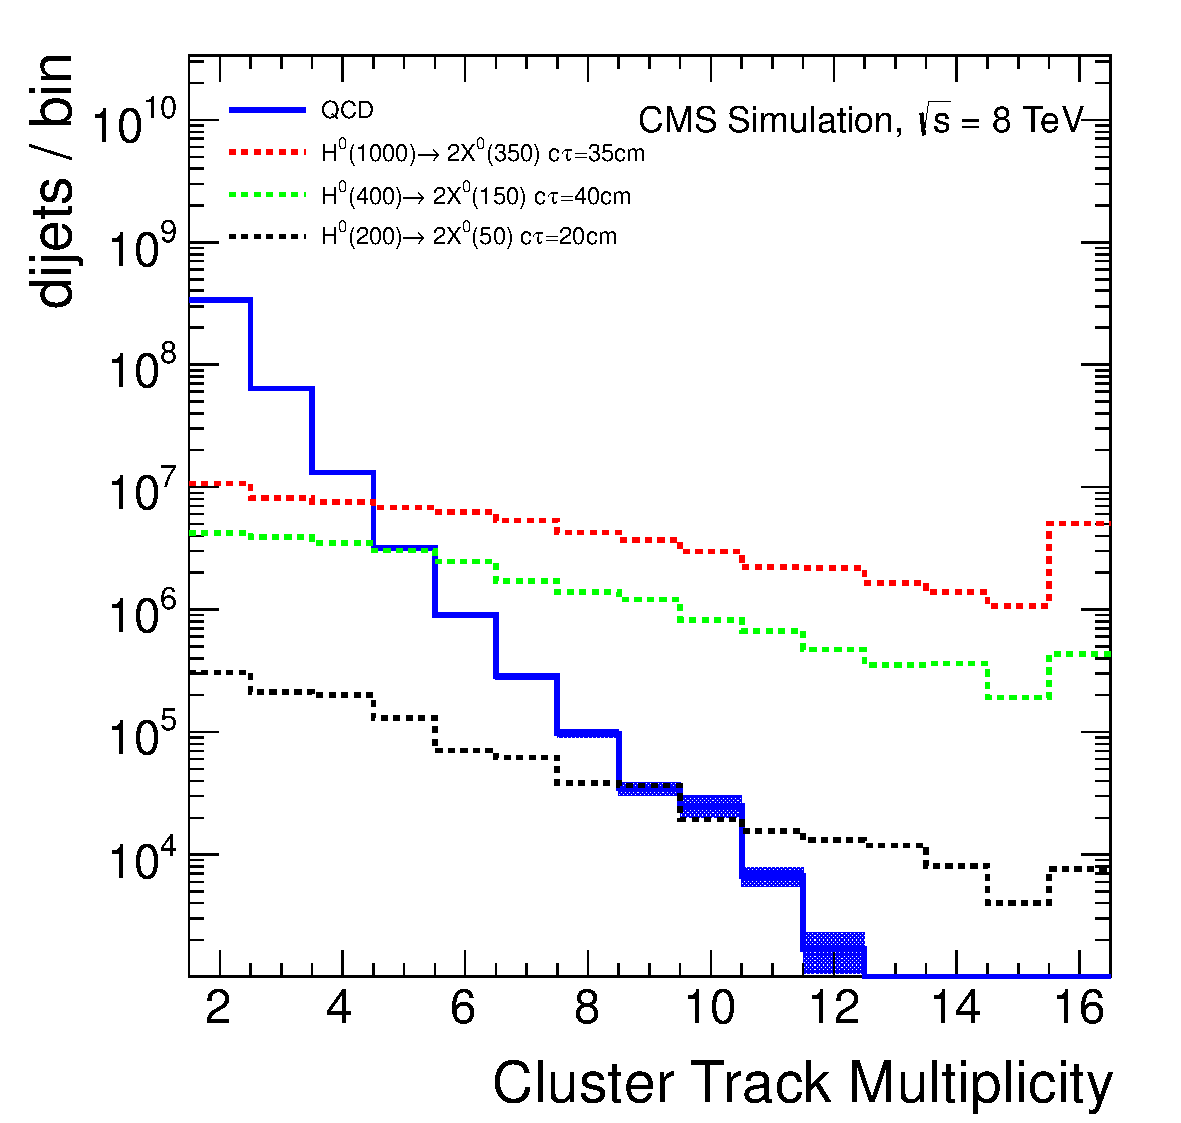
\includegraphics[width=0.49\textwidth]{plots/discrimination/disc_clrN.pdf}
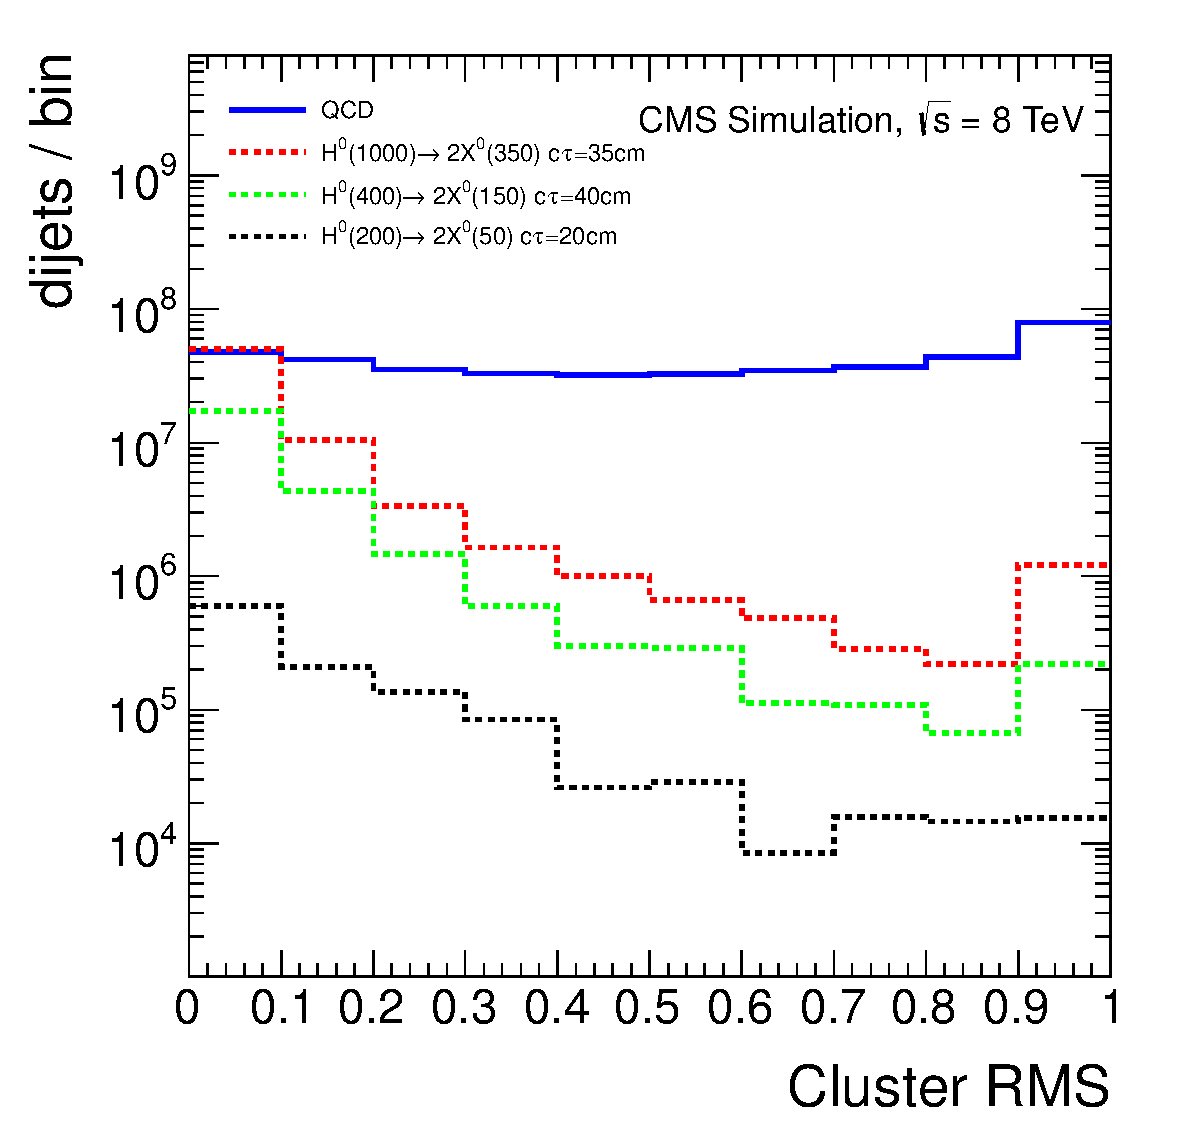
\includegraphics[width=0.49\textwidth]{plots/discrimination/disc_clrRMS.pdf}
\caption{Cluster discrimination variables for signal and background MC sample. \label{fig:discclr}}

\end{figure}


\end{enumerate}

\section{Selection}
\label{sec:selection}

To determine the background level, we use a data-driven technique
of independent selection criteria, the ``ABCD method", which is
 described in detail in Section \ref{sec:abcd}. This method requires
at least two selection criteria where the probability of a background candidate to pass one 
criterion is
not correlated with whether it passes the other criterion. Such selection criteria can be generally
constructed
from variables which are mutually independent. 
 In order to eliminate pairs of variables that are not independent,
 correlation factors have been studied using the background samples.  
Correlation factors between variables $x$ and $y$ are obtained from binned two-dimensional histograms 
according to the formula:
\begin{equation}
 \text{corr}(x,y) = \text{cov}(x,y)/\text{RMS}(x)\text{RMS}(y), \hspace{5pt} \text{cov}(x,y)= \sum_i(x_i y_i)/N - \sum_i(x_i)/N \sum_i(y_i)/N
\label{eqn:corr}
\end{equation}
where N is the normalization of the histogram and index $i$ loops over the histogram bins. Based on the study of the correlation factors, we construct
three independent selection criteria for the background estimation:

\begin{itemize}     
\item[1.] {\bf Combination of the number of prompt tracks and prompt tracks jet energy fraction selections} - for first jet in the dijet pair;
\item[2.] {\bf Combination of the number of prompt tracks and prompt tracks jet energy fraction selections} - for second jet in the dijet pair;
\item[3.] {\bf Combined vertex \& cluster likelihood discriminant}. 
We select variables that have small model dependence and are 
well uncorrelated with prompt tracks variables. They include:
\begin{itemize}
 \item vertex track multiplicity;
 \item fraction of tracks assigned to the vertex with positive value of signed transverse impact parameter;
 \item cluster track multiplicity;
 \item cluster RMS.
\end{itemize}  
The likelihood discriminant is obtained using signal and background MC samples, where samples for
various signal models are added together due to small signal dependence of the variables used.
For each dijet candidate a signal probability is computed according to the formula:
\begin{equation}
p=\frac{p_S}{p_S+p_B}=\frac{1}{1+p_B/p_S}=\frac{1}{1+\Pi_i p_B{}_i/p_S{}_i}
\label{eqn:likelihood}
\end{equation}
where the index $i$ loops over variables included in the discriminant. The correlations between individual variables 
within the discriminant are
neglected. Individual probability densities are determined 
using one-dimensional histograms for signal and background candidates separately.
\end{itemize}

As presented in Table \ref{tab:corr}, the individual correlation factors between the variables used for background
estimation do not exceed the few-percent level in the background MC samples.
There are large correlations between the number of prompt tracks and jet energy fraction carried by prompt tracks 
for the same jet, hence these two selections are applied together, while there is very little correlation for these
variables between the two jets that form the dijet pair. The choice of variables is
motivated by the independence of the prompt track variables between the two jets,
 while the variables associated with the secondary vertex use displaced tracks
from both jets simultaneously.

\begin{table}[htbp]
\centering
\caption{Correlation factors obtained with Eq. \ref{eqn:corr} between the variables 
used for background estimation obtained from background QCD MC
samples. N1 and N2 represent the numbers
of prompt tracks for jets 1 and 2, respectively, while fraction 1 and 2 the jet energy fraction carried by
prompt tracks.
\label{tab:corr}}
\begin{tabular}{c|ccccc}
 & Vtx/Cluster & N1 & N2 & fraction 1 & fraction 2 \\
\hline
Vtx/Cluster & - & 1.1\% & 2.5\% & -2.7\% & 1.8\%  \\
N1 & & - & 2.3\% & 26\%  & 1.2\% \\
N2 & & & - & 0.5\% & 31\% \\
fraction 1 & & & & - & 0.3\% \\
fraction 2 & & & & & - \\
\end{tabular}
\end{table}

The final numerical values required for the variables used for background estimation are described in Section 
\ref{sec:cutvalues}. For all remaining discrimination variables we require loose preselection criteria:   
\begin{itemize}
 \item vertex mass $>$ 4\GeV;
 \item vertex $p_T>$ 8\GeV;
 \item average number of missing tracker hits behind the secondary vertex position $\leq$ 2 per track;
 \item $L_{xy}$ significance $>$ 8.
\end{itemize}

The reconstruction and preselection procedure 
may result in multiple candidates per event that all pass
the preselection criteria. In such cases, we select only one candidate per event by
choosing the one with the highest number of tracks associated to the secondary vertex.
If two or more candidates have the same number of tracks associated to the secondary vertex,
we choose the candidate with a smaller $\chi^2/\text{dof}$. The candidate preselection together
with the selection of the 
one candidate per event will be further referred to as event preselection.
Only the 
properties of the one selected candidate are used for further selection and background estimation.
It is worth noting that
among the background MC events above 99\% of events contains only one candidate
after the preselection criteria are applied. 

%When a single jet is used in more than one dijet pair after preselection, we 
%In case a single jet is used in more than one dijet pair after preselection, we resolve
%the ambiguity by choosing the highest $L_{xy}$ significance candidate for each jet, thus ensuring that
%each jet is only used once. 

Preselection criteria efficiencies are presented in Table \ref{tab:seleff}.  
When the preselection requirements are applied to each dijet candidate,
the efficiencies are computed using the number of events with at least one candidate fulfilling the selection.
The requirement for the signal candidates to be matched with a decay of an \X boson at the generator level,
 denoted in Table \ref{tab:seleff} as {\it signal dijet}, 
is inefficient with respect to the trigger, if the two triggering
jets do not originate from the same \X boson particle.  
The $H_T>300\GeV$ requirement imposed by the trigger reduces the efficiency for lower masses of the \Higgs, 
while the vertex reconstruction efficiency is affected by the acceptance of the CMS tracker, which cannot 
reconstruct vertices displaced by more than 60\cm in the transverse plane. However, if the trigger accepted a signal event and the secondary vertex is reconstructed
for at least one of the \X boson candidates the preselection efficiency is high for the signal samples
when compared to the background.   

\begin{table}[!htbp]
\centering
\caption{Trigger and preselection criteria efficiency for data,
background MC, and three selected signal models. 
Event selection efficiencies in each row are relative to events that passed the criteria from rows above.
All criteria, except the trigger, are applied to individual dijet candidates.
There may be many dijet candidates in a single event, therefore
for those criteria the efficiency is computed using the number of events 
containing at least one dijet candidate that fulfills the selection. 
\label{tab:seleff}}
\begin{tabular}{|l|ccccc|}
\hline
 & \multicolumn{5}{c|}{preselection criteria efficiency} \\
\cline{2-6}
 & & &  $M_H$=1000\GeV & $M_H$=400\GeV & $M_H$=200\GeV \\
 & & &  $M_X$=350\GeV & $M_X$=150\GeV & $M_X$=50\GeV \\
selection & data & bkg. MC & $c\tau$=35\cm & $c\tau$=40\cm & $c\tau$=7\cm\\
\hline
trigger & - & 0.01\% & 97\% & 53\% & 3.9\% \\
has dijet & 99\% & 99\% & 100\% & 100\% & 99\% \\
signal dijet & - & - & 88\% & 65\% & 21\% \\
has vertex & 25\% & 24\% & 69\% & 59\% & 61\% \\
has cluster &  72\% & 72\% & 99\% & 98\% & 98\% \\
%\hline
vertex $\chi^2$ & 93\% & 93\% & 100\% & 99\% & 99\% \\
vertex mass &  78\% & 82\% & 98\% & 97\% & 74\% \\
vertex $p_T$ & 43\% & 42\% & 97\% & 95\% & 92\% \\
max missing hits & 8.5\% & 12\% & 98\% & 98\% & 98\%  \\
$L_{xy}$ significance & 78\% & 68\% & 100\% & 100\% & 100\% \\
\hline 
\end{tabular}
\end{table}

In order to validate the simulation based study, we compare the data and background MC distributions
in a control region for events passing the preselection.
We use a control region that requires passing the single jet trigger
 and vetoes events passing the double jet trigger (the single and double jet trigger
definitions are given in Section \ref{subsec:trigger}). Compared to the signal region, there is a factor of 100 less integrated 
luminosity and the signal efficiency for all considered signal models is at least ten 
times smaller than the efficiency
in the signal region. Figures \ref{fig:promptness}, \ref{fig:discriminant}, \ref{fig:vertex} 
and \ref{fig:cluster} present all 
of the discrimination variables used in the analysis in the control region
after event preselection. The number of missing hits per track after the vertex requirement has been removed
in order to increase the statistics of the 
data and background MC samples. 
Good agreement between data and background MC is found in most of the cases, suggesting
that background sources are well modeled in the MC simulation.

\begin{figure}[htbp]
\centering
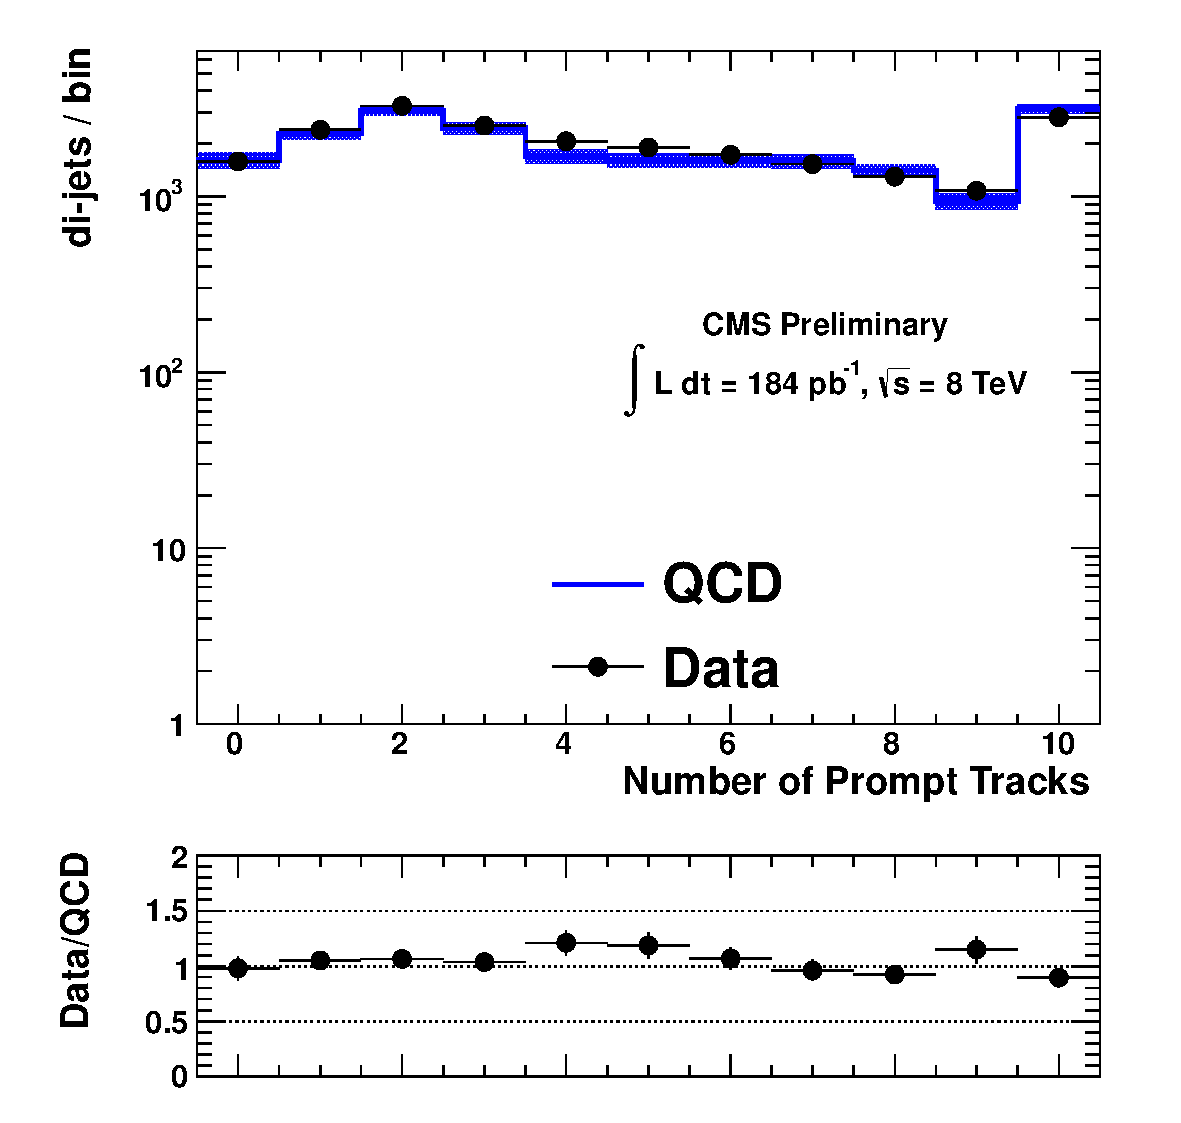
\includegraphics[width=0.49\textwidth]{plots/control/ctrl_NPromptTracks.pdf}
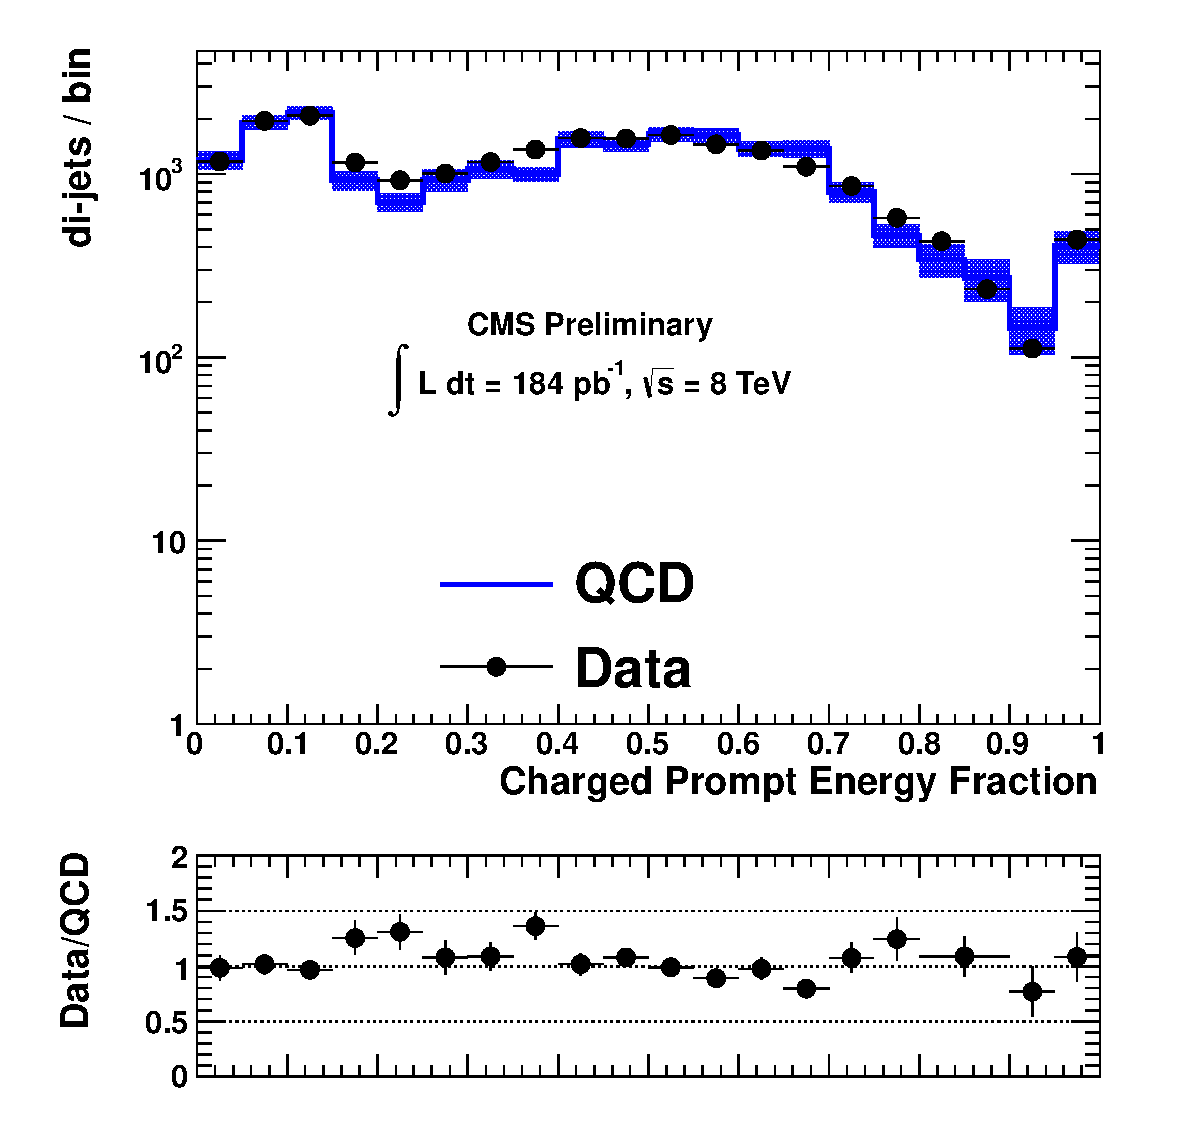
\includegraphics[width=0.49\textwidth]{plots/control/ctrl_PromptEnergyFrac.pdf}

\caption{Prompt track variables corresponding to the ones used in the trigger. 
The characteristic shape towards low values in both variables
shows the contribution of jets passing the non-prompt trigger requirement. \label{fig:promptness}}
\end{figure}

\begin{figure}[htbp]
\centering
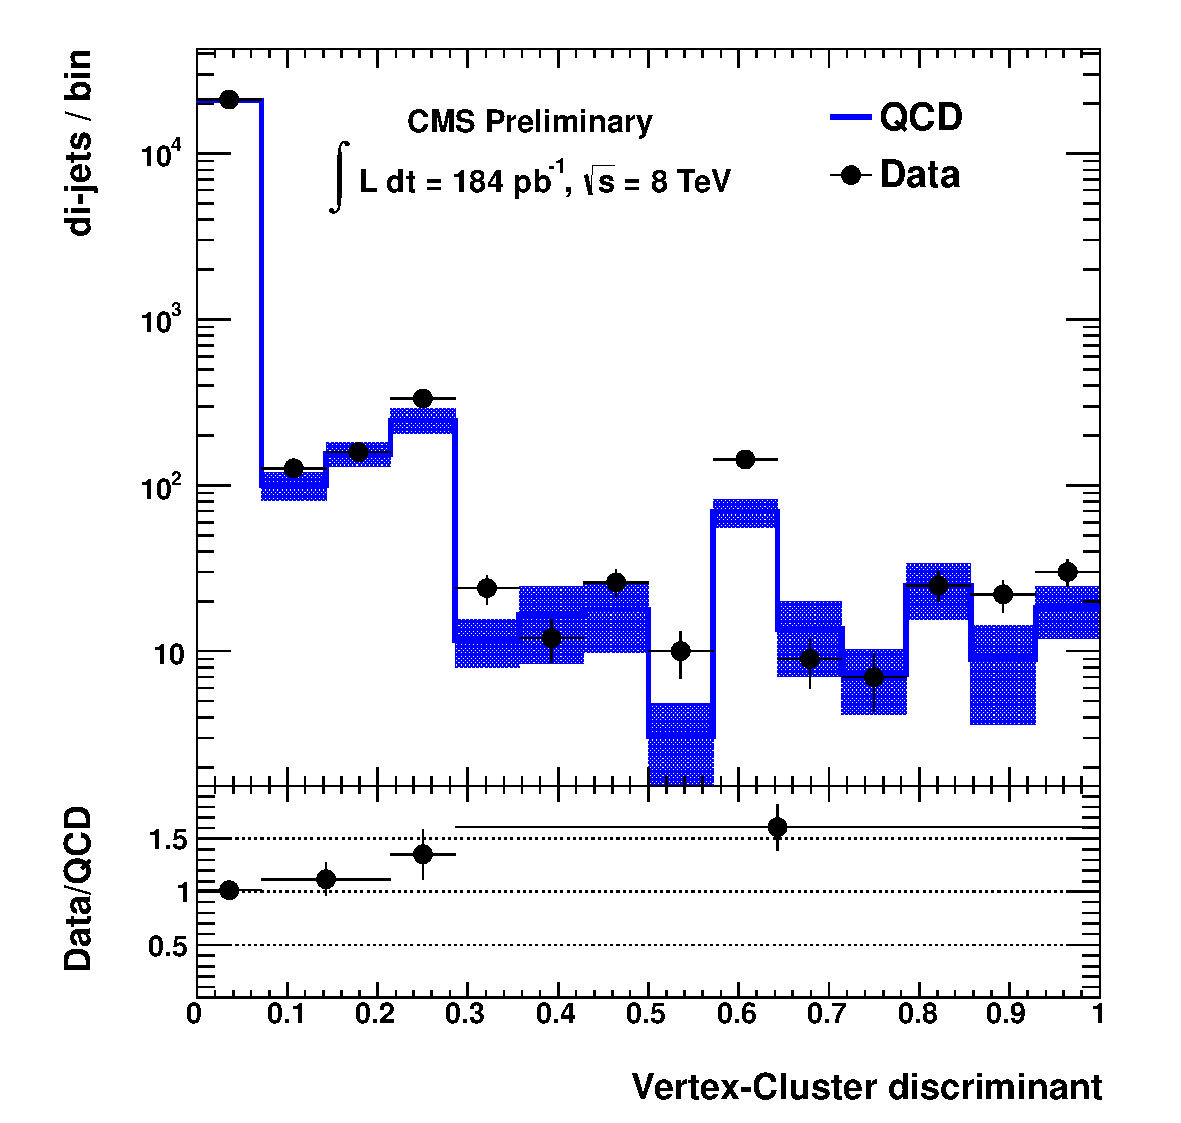
\includegraphics[width=0.49\textwidth]{plots/control/ctrl_Discriminant.pdf}
\caption{Vertex-Cluster likelihood discriminant.\label{fig:discriminant}}
\end{figure}

\begin{figure}[htbp]
\centering
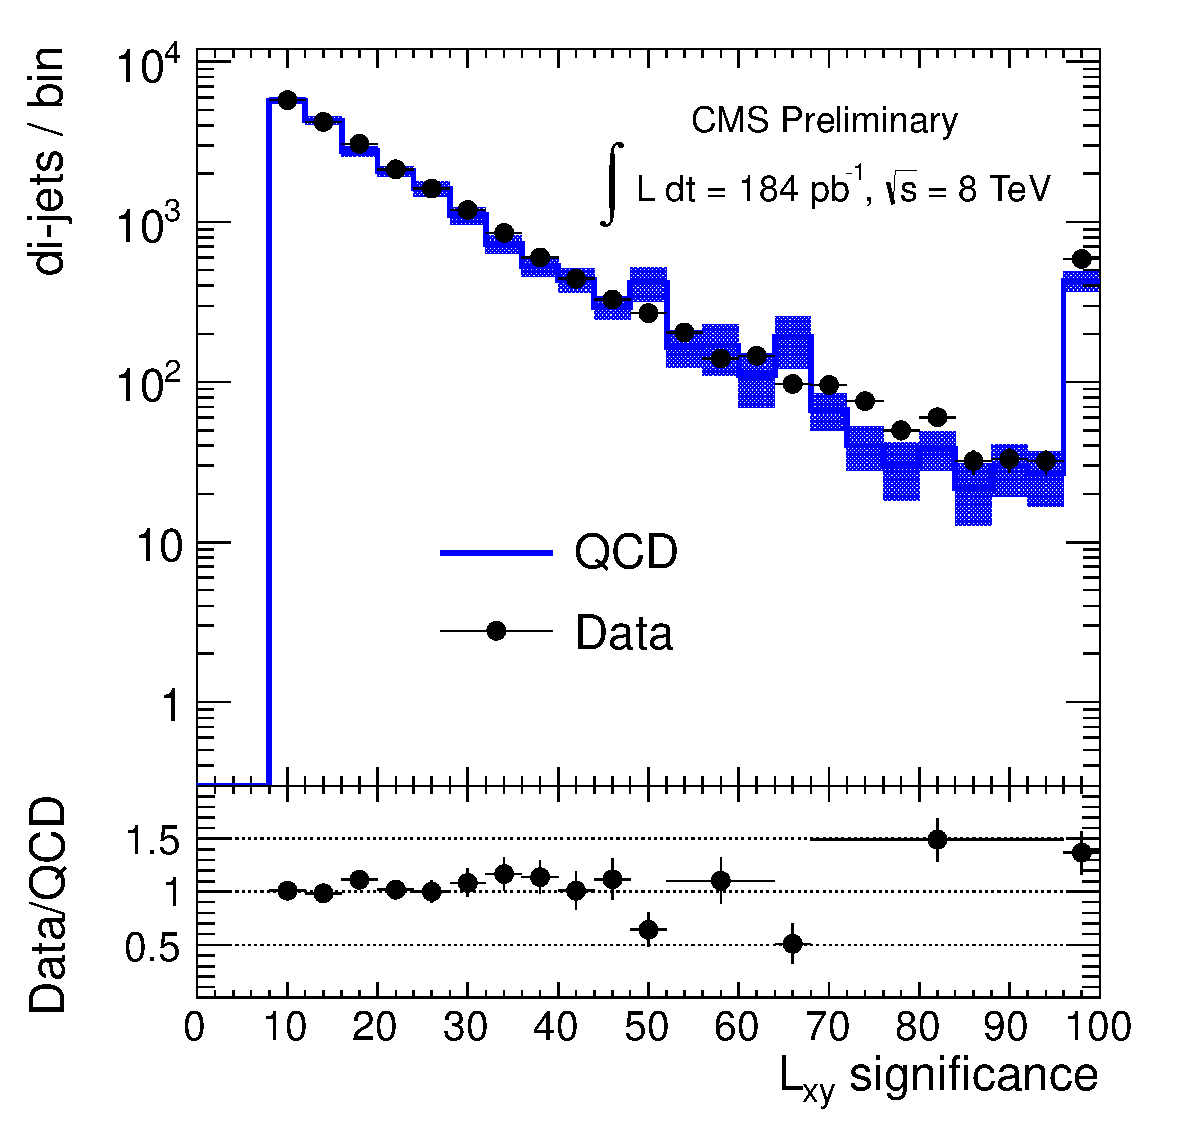
\includegraphics[width=0.49\textwidth]{plots/control/ctrl_Lxysig.pdf}
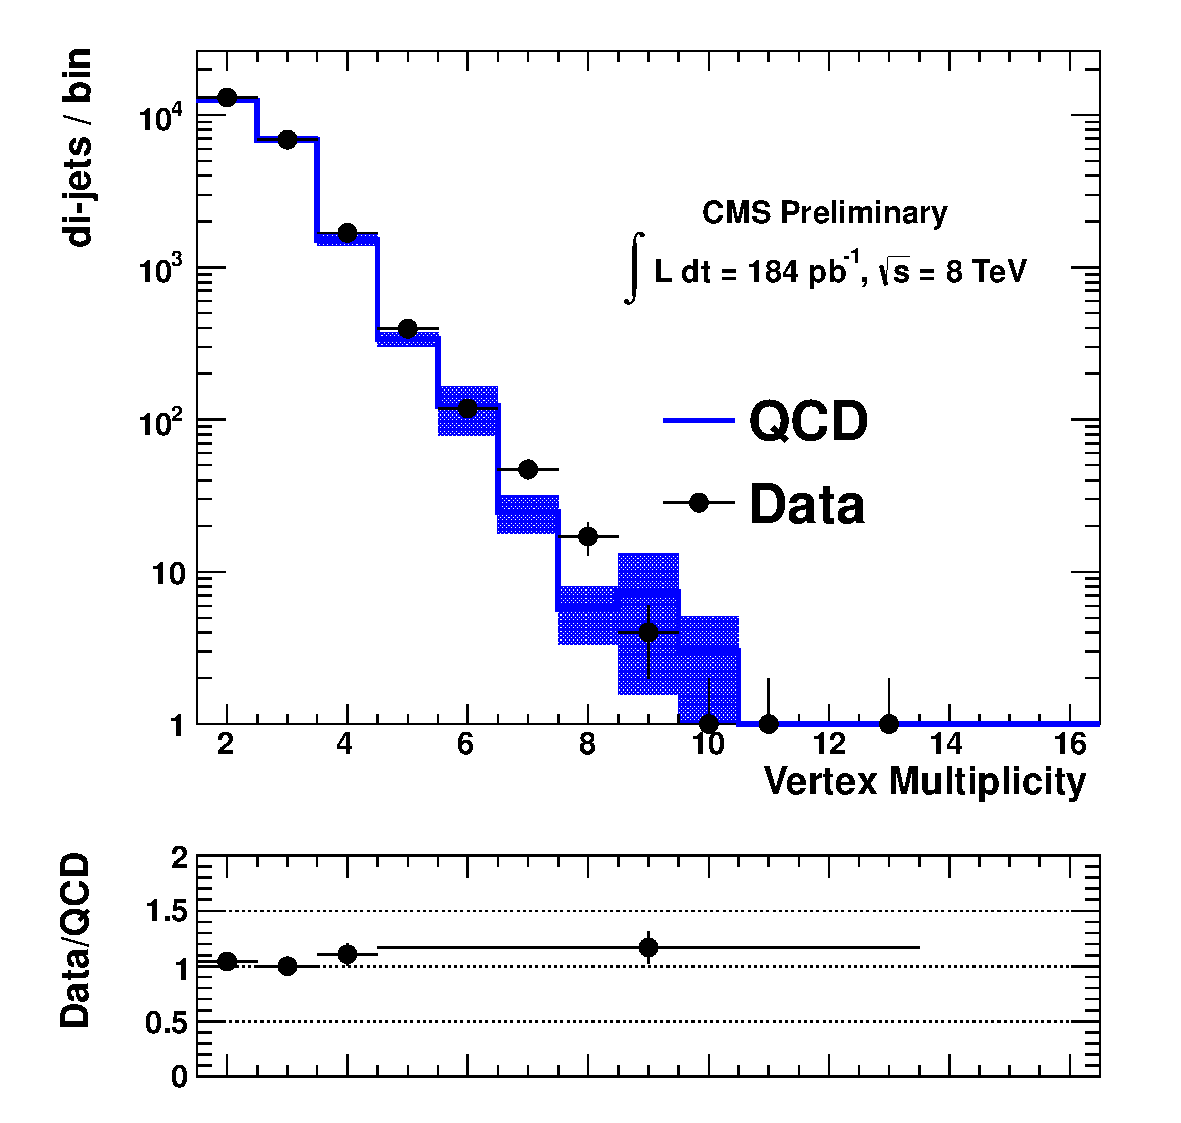
\includegraphics[width=0.49\textwidth]{plots/control/ctrl_VtxN.pdf}\\
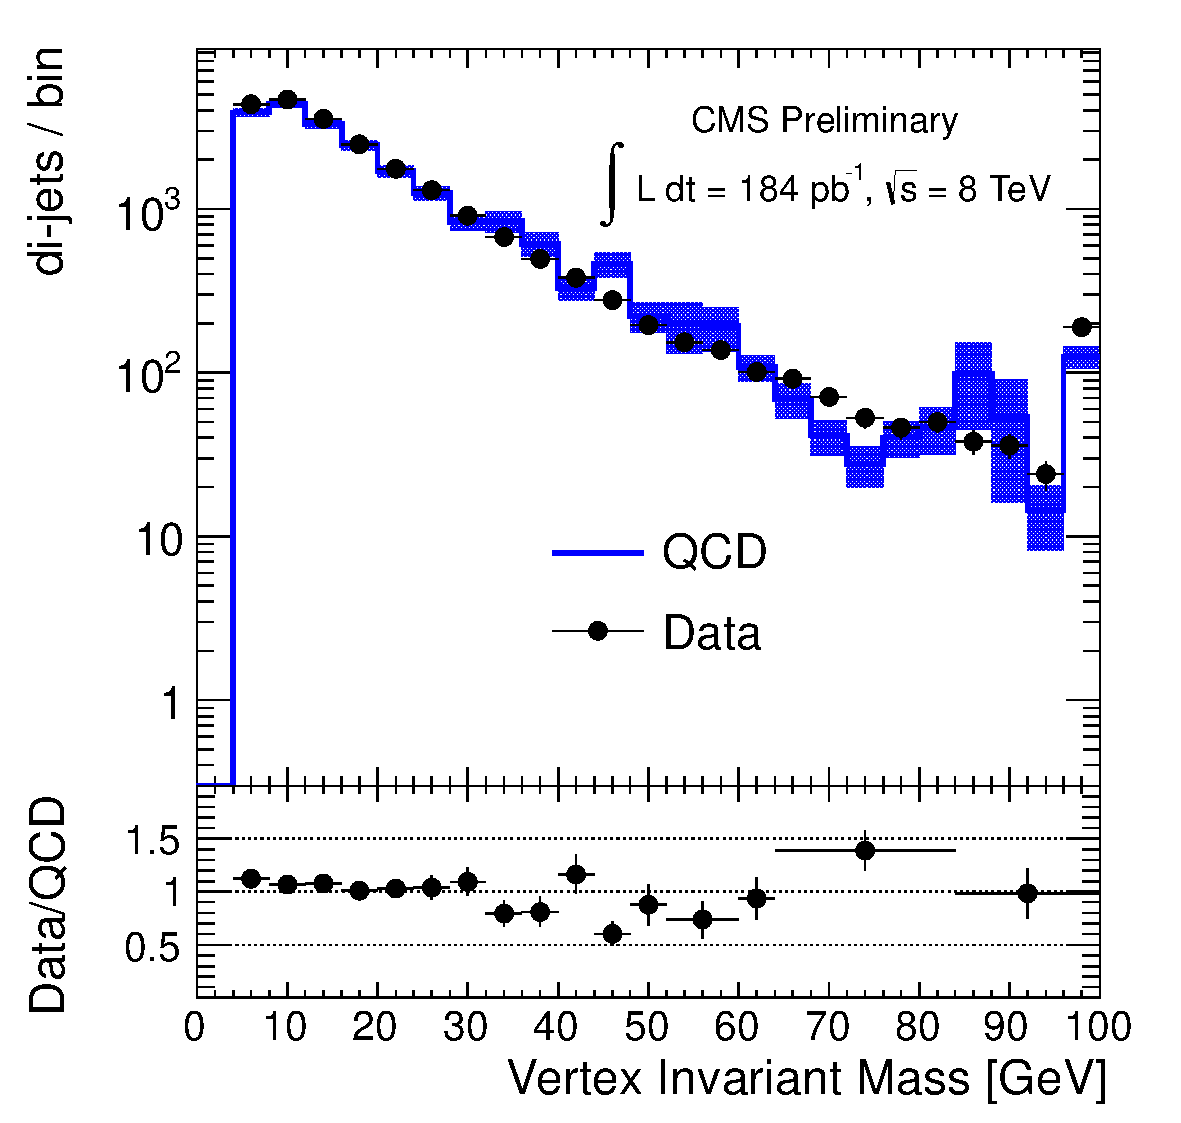
\includegraphics[width=0.49\textwidth]{plots/control/ctrl_Vtxmass.pdf}
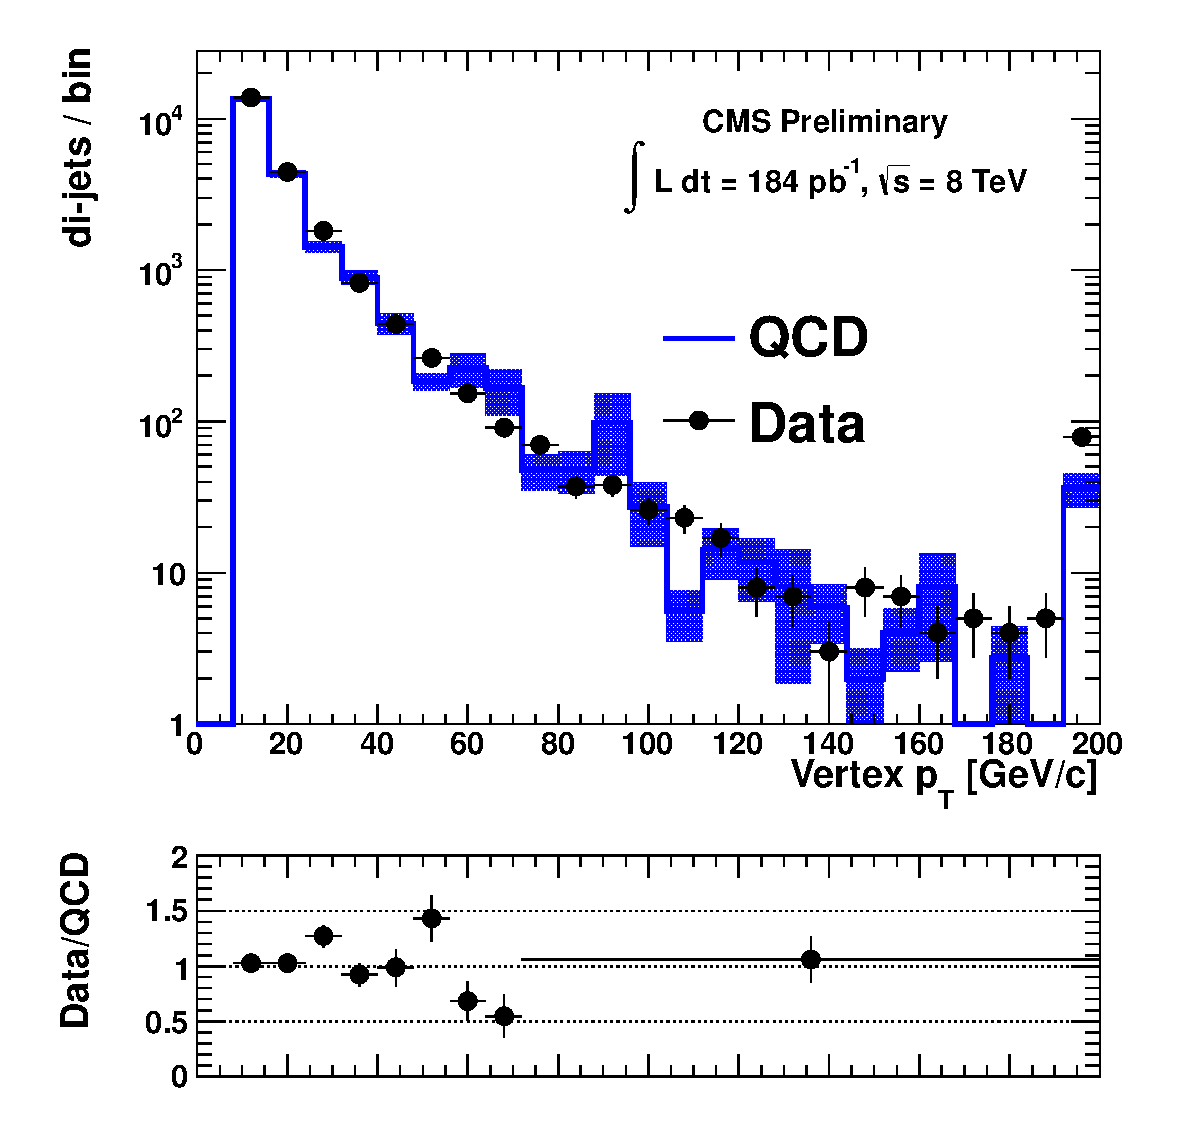
\includegraphics[width=0.49\textwidth]{plots/control/ctrl_Vtxpt.pdf}\\
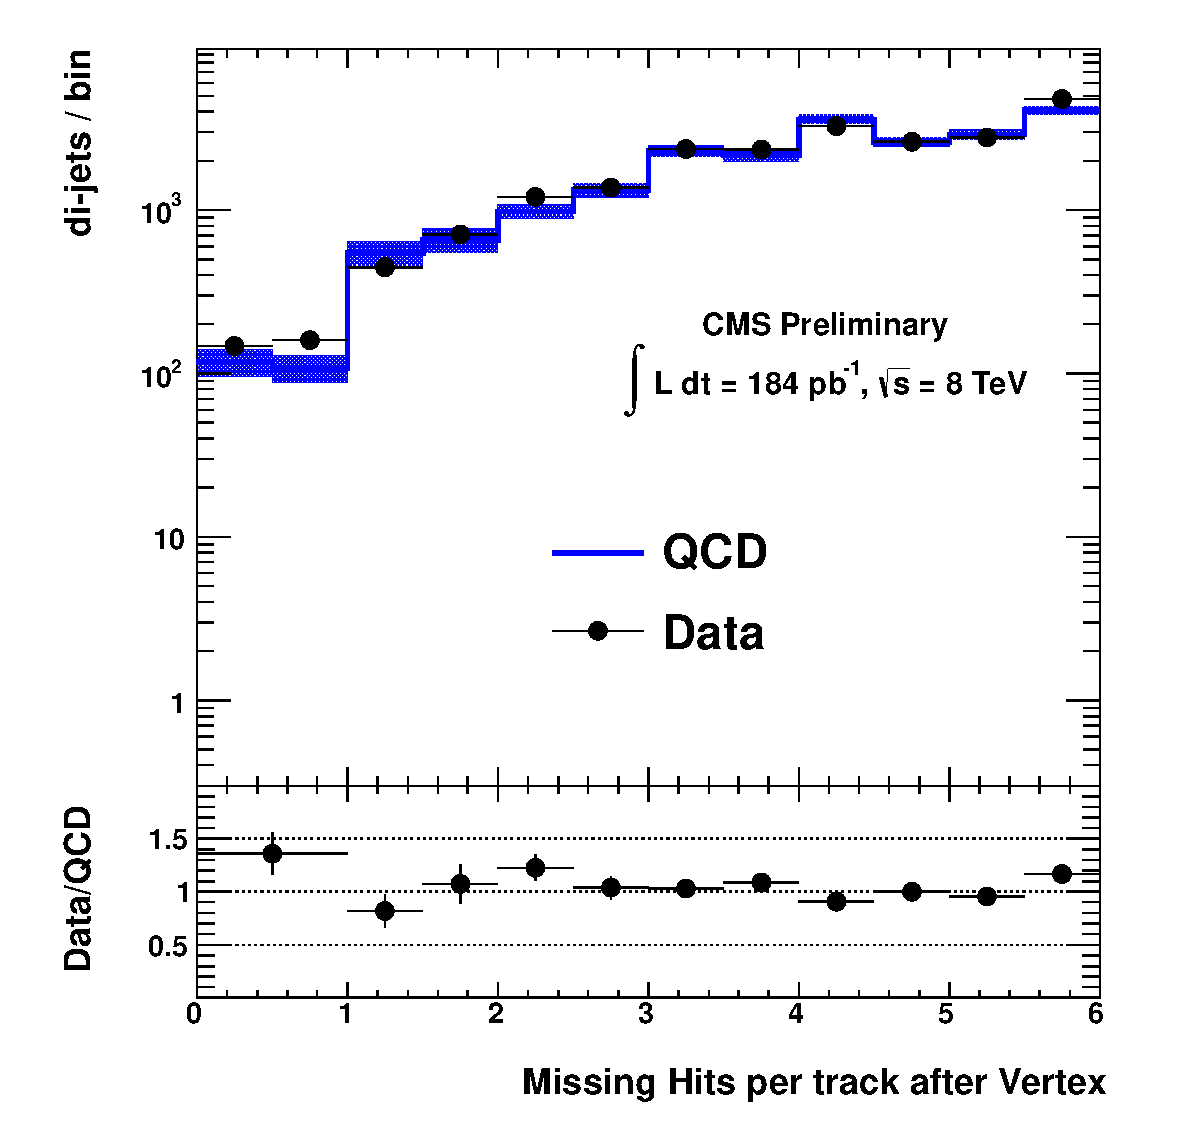
\includegraphics[width=0.49\textwidth]{plots/control/ctrl_NAvgMissHitsAfterVert.pdf}
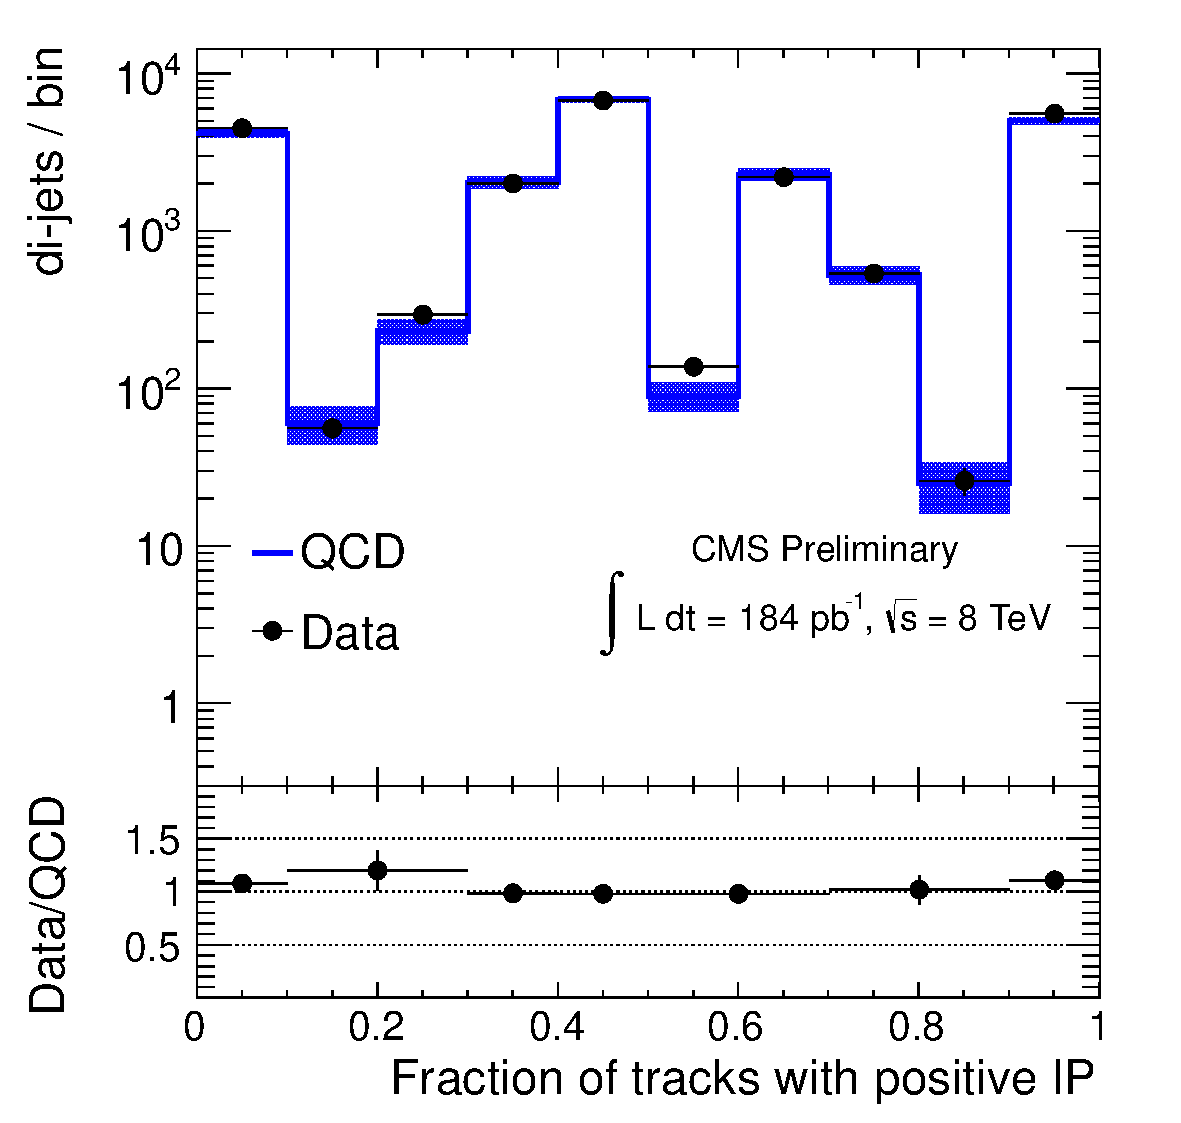
\includegraphics[width=0.49\textwidth]{plots/control/ctrl_Posip2dFrac.pdf}

\caption{Vertex variables. \label{fig:vertex}}
\end{figure}


\begin{figure}[htbp]
\centering
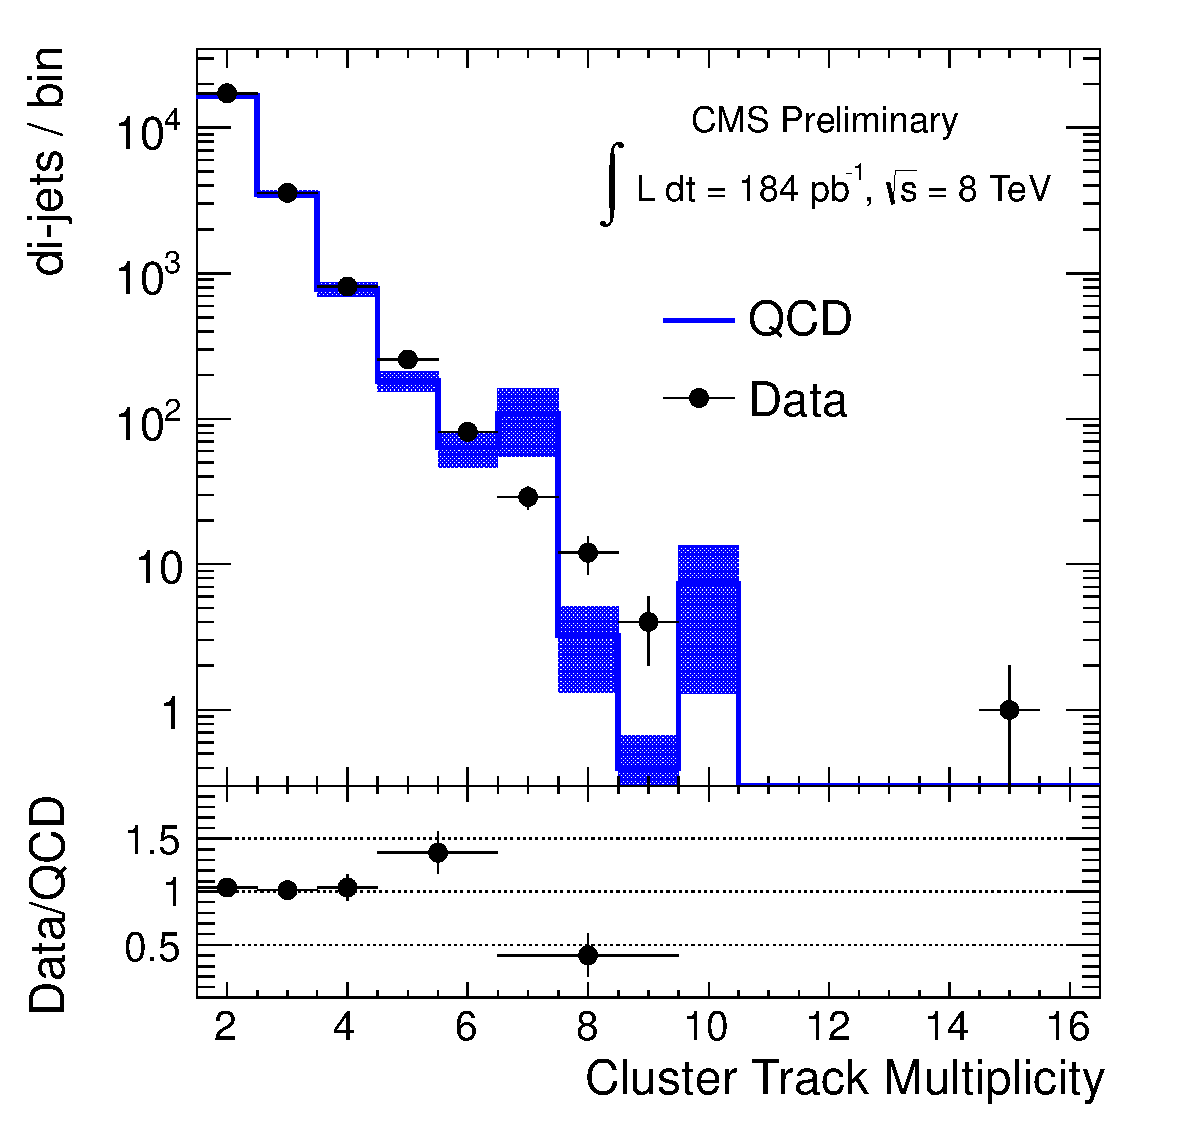
\includegraphics[width=0.49\textwidth]{plots/control/ctrl_clrN.pdf}
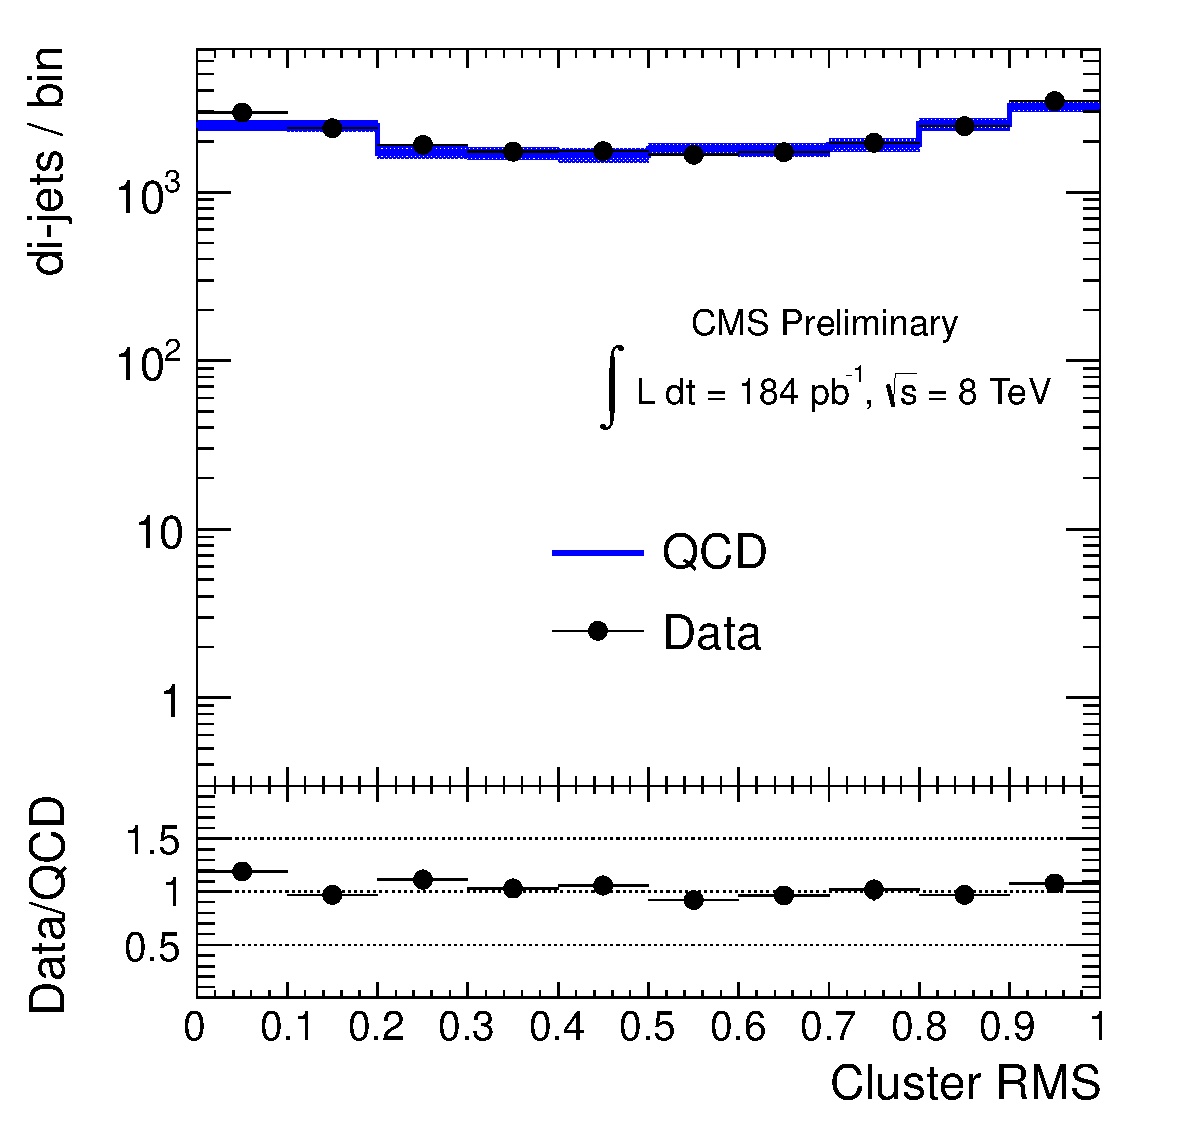
\includegraphics[width=0.49\textwidth]{plots/control/ctrl_clrRMS.pdf}

\caption{Cluster of $L_{xy}^\text{exp}$ variables. Candidates for which cluster RMS is above 1 do not share
tracks between the vertex and cluster reconstructions. \label{fig:cluster}}
\end{figure}

